\documentclass[hyperref,french,usenames,xcolor=dvipsnames]{beamer}
\mode<presentation>
{
\usepackage{beamerthemesplit}
\usetheme[compress,secheader]{Madrid}
\setbeamercovered{transparent}
}
%\usepackage{beamerarticle}

\usepackage{amsthm}
\usepackage{amsfonts}
\usepackage{amsmath}
\usepackage{graphicx}
\usepackage{color} 
%\usepackage{comment}
%\usepackage{epsfig}
\usepackage{xspace}
%\usepackage{stmaryrd}
%\usepackage{theorem} % Styles supplémentaires pour théorèmes
\usepackage{url}
\usepackage{array}  % Tableaux évolués
%\usepackage{multirow}  % Pour des colonnes sur plusieurs lignes
%\usepackage{soul}
%\usepackage{gastex}
\usepackage[latin1]{inputenc}   %accents 8 bits dans le source
%\usepackage[english]{algorithme}
%\usepackage[T1]{fontenc} %pour un beau PDF sous Linux ; � retirer sous Mac 
\usepackage[english]{babel}
\usepackage{tabularx}
%\usepackage{ulem}  % Pour l'attribut barre


%\usepackage[english]{babel}
%\usepackage{times}
%\usepackage[utf8]{inputenc}
%\usepackage{amssymb}
%\usepackage{movie15}
%\usepackage{graphicx,color} 
\usepackage{hyperref}


\usepackage{tikz}
\newdimen\pgfex
\newdimen\pgfem
\usetikzlibrary{arrows,shapes,shadows,scopes}
\usetikzlibrary{positioning}
\usetikzlibrary{matrix}
\usetikzlibrary{decorations.text}
\usetikzlibrary{decorations.pathmorphing}

% Macros relatives à la traduction de PH avec arcs neutralisants vers PH à k-priorités fixes

% Macros générales
\newcommand{\ie}{\textit{i.e.} }

% Notations générales pour PH
\newcommand{\PH}{\mathcal{PH}}
\newcommand{\PHs}{\mathcal{S}}
%\newcommand{\PHp}{\mathcal{P}}
\newcommand{\PHp}{\textcolor{red}{\mathcal{P}}}
\newcommand{\PHproc}{\mathcal{P}}
\newcommand{\PHa}{\mathcal{A}}
\newcommand{\PHl}{\mathcal{L}}
\newcommand{\PHn}{\mathcal{N}}

\newcommand{\PHfrappeur}{\mathsf{frappeur}}
\newcommand{\PHcible}{\mathsf{cible}}
\newcommand{\PHbond}{\mathsf{bond}}
\newcommand{\PHsorte}{\mathsf{sorte}}
\newcommand{\PHbloquant}{\mathsf{bloquante}}
\newcommand{\PHbloque}{\mathsf{bloquee}}

\newcommand{\PHfrappeR}{\textcolor{red}{\rightarrow}}
\newcommand{\PHmonte}{\textcolor{red}{\Rsh}}

\newcommand{\PHfrappeA}{\rightarrow}
\newcommand{\PHfrappeB}{\Rsh}
%\newcommand{\PHfrappe}[3]{\mbox{$#1\PHfrappeA#2\PHfrappeB#3$}}
%\newcommand{\PHfrappebond}[2]{\mbox{$#1\PHfrappeB#2$}}
\newcommand{\PHfrappe}[3]{#1\PHfrappeA#2\PHfrappeB#3}
\newcommand{\PHfrappebond}[2]{#1\PHfrappeB#2}
\newcommand{\PHobjectif}[2]{\mbox{$#1\PHfrappeB^*\!#2$}}
\newcommand{\PHconcat}{::}
\newcommand{\PHneutralise}{\rtimes}

\def\PHget#1#2{{#1[#2]}}
%\newcommand{\PHchange}[2]{#1\langle #2 \rangle}
\newcommand{\PHchange}[2]{(#1 \Lleftarrow #2)}
\newcommand{\PHarcn}[2]{\mbox{$#1\PHneutralise#2$}}
\newcommand{\PHjoue}{\cdot}

\newcommand{\PHetat}[1]{\mbox{$\langle #1 \rangle$}}

% Notations spécifiques aux graphes d'états
\newcommand{\PHge}{\textcolor{red}{\mathcal{GE}}}
\newcommand{\PHt}{\mathcal{T}}
\newcommand{\GE}{\mathcal{GE}}
\newcommand{\GEt}{\mathcal{T}}
\newcommand{\GEl}{\PHl}
\newcommand{\GEa}{\PHa}
\newcommand{\GEva}[3]{#1 \stackrel{#2}{\longrightarrow} #3}
\newcommand{\GEval}[3]{#1 \stackrel{#2}{\Longrightarrow} #3}
\newcommand{\GEget}[2]{\PHget{#1}{#2}}



% Notations pour le modèle de Thomas (depuis thèse)
\def\levels{\mathsf{niveaux}}
\def\levelsA#1#2{\levels_+(#1\rightarrow #2)}
\def\levelsI#1#2{\levels_-(#1\rightarrow #2)}
\newcommand{\PHres}{\mathsf{Res}}

% Notations spécifiques au modèle de Thomas
\newcommand{\Kinconnu}{\emptyset}
\newcommand{\RRGva}[3]{#1 \stackrel{#2}{\longrightarrow} #3}
\newcommand{\RRGgi}{\mathcal{G}}
\newcommand{\RRGreg}[1]{\RRGgi_{#1}}
\newcommand{\RRGres}[2]{\PHres_{#1}(#2)}



% Notations spécifiques aux actions conjointes
\newcommand{\PHfrappeAconjointe}{\rightarrowtail}
\newcommand{\PHfrappec}[3]{\mbox{$#1\PHfrappeAconjointe#2\PHfrappeB#3$}}



% Notations spécifiques à ce document
\newcommand{\A}{}
\newcommand{\B}{'}
%\newcommand{\A}{_A}
%\newcommand{\B}{_B}
\newcommand{\simule}{\rho}
\newcommand{\relsimule}{\textcolor{red}{\lesssim}}
\newcommand{\abstraction}{\alpha}
\newcommand{\chap}[1]{\textcolor{blue}{\widehat{#1}}}

% Notations spécifiques à la traduction
\newcommand{\PHsc}{\ensuremath{sc}}
\newcommand{\PHsca}[1]{\ensuremath{\PHsc^{#1}}}
\newcommand{\PHfsc}{f_{sc}}
\newcommand{\PHjouables}{\mathsf{jouables}}

\usepackage{ifthen}
\usepackage{tikz}
\usetikzlibrary{arrows,shapes}

\definecolor{lightgray}{rgb}{0.8,0.8,0.8}
\definecolor{lightgrey}{rgb}{0.8,0.8,0.8}

\tikzstyle{boxed ph}=[]
\tikzstyle{sort}=[fill=lightgray,rounded corners]
\tikzstyle{process}=[circle,draw,minimum size=15pt,fill=white,
font=\footnotesize,inner sep=1pt]
\tikzstyle{black process}=[process, fill=black,text=white, font=\bfseries]
\tikzstyle{gray process}=[process, draw=black, fill=lightgray]
\tikzstyle{current process}=[process, draw=black, fill=lightgray]
\tikzstyle{process box}=[white,draw=black,rounded corners]
\tikzstyle{tick label}=[font=\footnotesize]
\tikzstyle{tick}=[black,-]%,densely dotted]
\tikzstyle{hit}=[->,>=angle 45]
\tikzstyle{selfhit}=[min distance=30pt,curve to]
\tikzstyle{bounce}=[densely dotted,>=stealth',->]
\tikzstyle{hl}=[font=\bfseries,very thick]
\tikzstyle{hl2}=[hl]
\tikzstyle{nohl}=[font=\normalfont,thin]

\newcommand{\currentScope}{}
\newcommand{\currentSort}{}
\newcommand{\currentSortLabel}{}
\newcommand{\currentAlign}{}
\newcommand{\currentSize}{}

\newcounter{la}
\newcommand{\TSetSortLabel}[2]{
  \expandafter\repcommand\expandafter{\csname TUserSort@#1\endcsname}{#2}
}
\newcommand{\TSort}[4]{
  \renewcommand{\currentScope}{#1}
  \renewcommand{\currentSort}{#2}
  \renewcommand{\currentSize}{#3}
  \renewcommand{\currentAlign}{#4}
  \ifcsname TUserSort@\currentSort\endcsname
    \renewcommand{\currentSortLabel}{\csname TUserSort@\currentSort\endcsname}
  \else
    \renewcommand{\currentSortLabel}{\currentSort}
  \fi
  \begin{scope}[shift={\currentScope}]
  \ifthenelse{\equal{\currentAlign}{l}}{
    \filldraw[process box] (-0.5,-0.5) rectangle (0.5,\currentSize-0.5);
    \node[sort] at (-0.2,\currentSize-0.4) {\currentSortLabel};
   }{\ifthenelse{\equal{\currentAlign}{r}}{
     \filldraw[process box] (-0.5,-0.5) rectangle (0.5,\currentSize-0.5);
     \node[sort] at (0.2,\currentSize-0.4) {\currentSortLabel};
   }{
    \filldraw[process box] (-0.5,-0.5) rectangle (\currentSize-0.5,0.5);
    \ifthenelse{\equal{\currentAlign}{t}}{
      \node[sort,anchor=east] at (-0.3,0.2) {\currentSortLabel};
    }{
      \node[sort] at (-0.6,-0.2) {\currentSortLabel};
    }
   }}
  \setcounter{la}{\currentSize}
  \addtocounter{la}{-1}
  \foreach \i in {0,...,\value{la}} {
    \TProc{\i}
  }
  \end{scope}
}

\newcommand{\TTickProc}[2]{ % pos, label
  \ifthenelse{\equal{\currentAlign}{l}}{
    \draw[tick] (-0.6,#1) -- (-0.4,#1);
    \node[tick label, anchor=east] at (-0.55,#1) {#2};
   }{\ifthenelse{\equal{\currentAlign}{r}}{
    \draw[tick] (0.6,#1) -- (0.4,#1);
    \node[tick label, anchor=west] at (0.55,#1) {#2};
   }{
    \ifthenelse{\equal{\currentAlign}{t}}{
      \draw[tick] (#1,0.6) -- (#1,0.4);
      \node[tick label, anchor=south] at (#1,0.55) {#2};
    }{
      \draw[tick] (#1,-0.6) -- (#1,-0.4);
      \node[tick label, anchor=north] at (#1,-0.55) {#2};
    }
   }}
}
\newcommand{\TSetTick}[3]{
  \expandafter\repcommand\expandafter{\csname TUserTick@#1_#2\endcsname}{#3}
}

\newcommand{\myProc}[3]{
  \ifcsname TUserTick@\currentSort_#1\endcsname
    \TTickProc{#1}{\csname TUserTick@\currentSort_#1\endcsname}
  \else
    \TTickProc{#1}{#1}
  \fi
  \ifthenelse{\equal{\currentAlign}{l}\or\equal{\currentAlign}{r}}{
    \node[#2] (\currentSort_#1) at (0,#1) {#3};
  }{
    \node[#2] (\currentSort_#1) at (#1,0) {#3};
  }
}
\newcommand{\TSetProcStyle}[2]{
  \expandafter\repcommand\expandafter{\csname TUserProcStyle@#1\endcsname}{#2}
}
\newcommand{\TProc}[1]{
  \ifcsname TUserProcStyle@\currentSort_#1\endcsname
    \myProc{#1}{\csname TUserProcStyle@\currentSort_#1\endcsname}{}
  \else
    \myProc{#1}{process}{}
  \fi
}

\newcommand{\repcommand}[2]{
  \providecommand{#1}{#2}
  \renewcommand{#1}{#2}
}
\newcommand{\THit}[5]{
  \path[hit] (#1) edge[#2] (#3#4);
  \expandafter\repcommand\expandafter{\csname TBounce@#3@#5\endcsname}{#4}
}
\newcommand{\TBounce}[4]{
  (#1\csname TBounce@#1@#3\endcsname) edge[#2] (#3#4)
}

\newcommand{\TState}[1]{
  \foreach \proc in {#1} {
    \node[current process] (\proc) at (\proc.center) {};
  }
}

% procedure, abstractions and dependencies
\newcommand{\abstr}[1]{#1^\wedge}%\text{\textasciicircum}}
\def\aBS{\abstr{\BS}}
\def\abeta{\abstr{\beta}}
\def\aZ{\abstr{\zeta}}
\def\aY{\abstr{\xi}}

\def\beforeproc{\vartriangleleft}

\def\powerset{\wp}

\def\Sce{\mathbf{Sce}}
\def\OS{\mathbf{OS}}
\def\Obj{\mathbf{Obj}}
\def\Proc{\mathbf{Proc}}

\usepackage{galois}
\newcommand{\theOSabstr}{toOS}
\newcommand{\OSabstr}[1]{\theOSabstr(#1)}
\newcommand{\theOSconcr}{toSce}
\newcommand{\OSconcr}[1]{\theOSconcr(#1)}

% \def\gO{\mathbb{O}}
% \def\gS{\mathbb{S}}
\def\aS{\mathcal{A}}
\def\Req{\mathrm{Req}}
\def\Sol{\mathrm{Sol}}
\def\Cont{\mathrm{Cont}}
\def\cBS{\BS_\ctx}
\def\caBS{\aBS_\ctx}
\def\caS{\aS_\ctx}
\def\cSol{\Sol_\ctx}
\def\cReq{\Req_\ctx}
\def\cCont{\Cont_\ctx}

\def\any{\star}

% \def\gProc{\mathrm{maxPROC}}
\def\mCtx{\mathrm{maxCtx}}

\def\procs{\f{procs}}
\def\objs{\f{objs}}
\def\sat#1{\lceil #1\rceil}

\def\gCont{\f{maxCont}}
\def\lCont{\f{minCont}}
\def\lProc{\f{minProc}}
\def\gProc{\f{maxProc}}

\def\join{\oplus}
\def\concat{\!::\!}
\def\ltw{\preccurlyeq_{\OS}}
\def\indexes#1{\mathbb{I}^{#1}}
%\def\indexes#1{\{1..|#1|\}}
\def\supp{\f{support}}
\def\w{\omega}
\def\W{\Omega}
\def\ctx{\varsigma}
\def\Ctx{\mathbf{Ctx}}
\def\mconcr{\gamma}
\def\concr{\mconcr_\ctx}
\def\obj#1#2{{#1\!\Rsh^*\!\!#2}}
\def\objp#1#2#3{\obj{{#1}_{#2}}{{#1}_{#3}}}
\def\A{\mathcal{A}}
\def\cwA{\A_\ctx^\w}
\def\cwReq{\Req_\ctx^\w}
\def\cwSol{\Sol_\ctx^\w}
\def\cwCont{\Cont_\ctx^\w}
\def\gCtx{\f{maxCtx}}
\def\endCtx{\f{endCtx}}
\def\ceil{\f{end}}

\def\lfp{\mathrm{lfp}\;}
\def\mlfp#1{\mathrm{lfp}\{#1\}\;}
\def\maxobjs{{\f{maxobjs}}}
\def\maxprocs{{\f{maxprocs}_\ctx}}
\def\objends{{\f{ends}}}

\def\ra{\rho}
\def\rb{\rho^\wedge}
\def\rc{\widetilde{\rho}}
\def\interleave{\f{interleave}}

\def\join{\concat}

\def\Pint{\textsc{PINT}}
\def\PH{\mathcal{PH}}

\tikzstyle{sort}=[fill=lightgray, rounded corners, draw=black]
\tikzstyle{process}=[circle,draw,minimum size=15pt,font=\footnotesize,inner sep=1pt]
\tikzstyle{black process}=[process, draw=blue, fill=red,text=black,font=\bfseries]
\tikzstyle{highlighted process}=[current process, fill=gray]
\tikzstyle{process box}=[fill=none,draw=black,rounded corners]
\tikzstyle{current process}=[process,fill=blue]
\tikzstyle{tick label}=[font=\footnotesize]
\tikzstyle{tick}=[densely dotted]
\tikzstyle{hit}=[->,>=angle 45]
\tikzstyle{selfhit}=[min distance=30pt,curve to]
\tikzstyle{bounce}=[densely dotted,>=stealth',->]
\tikzstyle{hlhit}=[very thick]
\tikzstyle{ulhit}=[draw=lightgray,fill=lightgray]
\tikzstyle{pulhit}=[fill=lightgray]
\tikzstyle{bulhit}=[draw=lightgray]

\tikzstyle{hitless graph}=[every edge/.style={draw=red,-}]

\tikzstyle{aS}=[every edge/.style={draw,->}]
\tikzstyle{Asol}=[draw,circle,minimum size=5pt,inner sep=0]
\tikzstyle{Aproc}=[draw]
\tikzstyle{Aobj}=[]

\renewcommand{\TState}[2]{
  \foreach \proc in {#2} {
        \only<#1>{ \node[current process] (\proc) at (\proc.center) {}; }
  };
}

\definecolor{darkgreen}{rgb}{0,0.5,0}
\definecolor{darkyellow}{rgb}{0.5,0.5,0}
\definecolor{lightyellow}{rgb}{1,1,0.6}
\definecolor{darkcyan}{rgb}{0,0.6,0.6}
\definecolor{darkorange}{rgb}{0.8,0.2,0}
\definecolor{newcolor}{rgb}{0, 0, .90}
\definecolor{impcolor}{rgb}{.90, 0, 0}
\definecolor{darkergreen}{rgb}{0,0.5,0}
\definecolor{myorange}{rgb}{0.8,0.7,0}
\definecolor{myviolet}{rgb}{0.7,0.0,0.7}
\definecolor{lightgray}{rgb}{0.8,0.8,0.8}
\definecolor{lightgrey}{rgb}{0.8,0.8,0.8}
\definecolor{darkred}{rgb}{0.5,0,0}
\definecolor{lightred}{rgb}{1,0.8,0.8}
\definecolor{lightgreen}{rgb}{0.7,1,0.7}
\definecolor{darkblue}{rgb}{0,0,0.5}

\definecolor{notsodarkgreen}{rgb}{0,0.7,0}
\colorlet{colorb}{blue}
\colorlet{colora1}{yellow}
\colorlet{colora0}{green}
\colorlet{colora1font}{darkyellow}
\colorlet{colora0font}{darkgreen}

\colorlet{exanswer}{blue}
\colorlet{colorgray}{lightgray}

\definecolor{colortitle}{rgb}{0.54,0.8,0.9}

%\definecolor{coloract}{rgb}{0,1,0}
%\definecolor{colorinh}{rgb}{1,0,0}
\colorlet{coloract}{darkgreen}
\colorlet{colorinh}{red}
\colorlet{coloractgray}{lightgreen}
\colorlet{colorinhgray}{lightred}
\colorlet{colorinf}{darkgray}
\colorlet{coloractgray}{lightgreen}
\colorlet{colorinhgray}{lightred}
\colorlet{light}{gray}


\definecolor{lightpurple}{rgb}{0.83,0.27,1}
\definecolor{lightblue}{rgb}{0.27,0.9,0.9}

%\definecolor{coloract}{rgb}{0,1,0}
%\definecolor{colorinh}{rgb}{1,0,0}
\colorlet{coloract}{darkgreen}
\colorlet{colorinh}{red}

\colorlet{couleurtheme}{darkblue}  % Couleur principale du thème
\usecolortheme[named=couleurtheme]{structure}    % Couleur de la structure : titres et puces
%\setbeamercolor{normal text}{bg=black,fg=white}  % Couleur du texte
\setbeamercolor{item}{fg=couleurtheme}           % Couleur des puces
\newcommand{\f}{\textcolor{couleurtheme}{\textbf{$\rightarrow$\ }}}

\tikzstyle{grn}=[every node/.style={circle,draw=black,outer sep=2pt,minimum
                size=15pt,text=black}, node distance=1.5cm]
\tikzstyle{inh}=[>=|,-|,draw=colorinh,thick, text=black,label]
\tikzstyle{act}=[->,>=triangle 60,draw=coloract,thick,color=coloract]
\tikzstyle{inhgray}=[>=|,-|,draw=colorinhgray,thick, text=black,label]
\tikzstyle{actgray}=[->,>=triangle 60,draw=coloractgray,thick,color=coloractgray]
\tikzstyle{inf}=[->,draw=colorinf,thick,color=colorinf]
%\tikzstyle{elabel}=[fill=none, above=-1pt, sloped,text=black, minimum size=10pt, outer sep=0, font=\scriptsize,draw=none]
\tikzstyle{elabel}=[fill=none,text=black, above=-2pt,%sloped,
minimum size=10pt, outer sep=0, font=\scriptsize, draw=none]
%\tikzstyle{elabel}=[]


\tikzstyle{plot}=[every path/.style={-}]
\tikzstyle{axe}=[gray,->,>=stealth']
\tikzstyle{ticks}=[font=\scriptsize,every node/.style={gray}]
\tikzstyle{mean}=[thick]
\tikzstyle{interval}=[line width=5pt,red,draw opacity=0.7]
\definecolor{lightred}{rgb}{1,0.3,0.3}

\tikzstyle{hl}=[yellow]
\tikzstyle{hl2}=[orange]

\tikzstyle{every matrix}=[ampersand replacement=\&]
\tikzstyle{shorthandoff}=[]
\tikzstyle{shorthandon}=[]
%%%%%%%%%%%%%%%%%%%%%%%%%%%%%%%%%%%%%%%%

% Environnement liste avec flèches
\newenvironment{fleches}{%
\begin{list}{}{%
\setlength{\labelwidth}{1em}% largeur de la boîte englobant le label
\setlength{\labelsep}{0pt}% espace entre paragraphe et l’étiquette
%\setlength{\itemsep}{1pt}
%\setlength{\leftmargin}{\labelwidth+\labelsep}% marge de gauche
\renewcommand{\makelabel}{\f}%
}}{\end{list}}

% Liste sans puce
\newenvironment{liste}{%
\begin{list}{}{%
\setlength{\labelwidth}{0em}% largeur de la boîte englobant le label
\setlength{\labelsep}{0pt}% espace entre paragraphe et l’étiquette
\setlength{\leftmargin}{0em}% marge de gauche
%\renewcommand{\makelabel}{\f}%
}}{\end{list}}


\newcommand{\texthl}[1]{{\color{red}#1}}
\newcommand{\jaune}[1]{{\color{red}#1}}
\newcommand{\texthlb}[1]{{\color{orange}#1}}
\newcommand{\orange}[1]{{\color{orange}#1}}
\newcommand{\verte}[1]{{\color{green}#1}}
\newcommand{\trad}{{\color{orange}{\bf $\leadsto$}}}

\newcommand{\textcite}[1]{{\color{myviolet}[#1]}}
\newcommand{\textciten}[1]{{\color{myviolet}#1}}
\newcommand{\tscite}[1]{\textcolor{couleurcit}{#1}}
%\newcommand{\tcite}[1]{\textcolor{couleurcit}{[#1]}}
\newcommand{\tcite}[1]{\textcolor{couleurcit}{[#1]}}

% Un vrai symbole pour l'ensemble vide
\renewcommand{\emptyset}{\varnothing}

% Pour définir la conférence et son nom court
\newcommand{\conference}[2]{\def\theconference{#2}
\def\insertshortconference{\ifthenelse{\equal{#1}{-}}{#2}{\ifthenelse{\equal{#1}{}}{#2}{#1}}}}


\newcommand{\New}[1]{\textcolor{newcolor}{#1}}
\newcommand{\Imp}[1]{\textcolor{impcolor}{#1}}
\newcommand{\setpns}{\textsl{Scheduling}-TPNs}
\newcommand{\ptpns}{\textsl{Preemptive}-TPNs}
\newcommand{\fihtpns}{FIHTPNs}
\newcommand{\setpn}{\textsl{Scheduling}-TPN}
\newcommand{\ptpn}{\textsl{Preemptive}-TPN}
\newcommand{\fihtpn}{FIHTPN}
\newcommand{\post}[1]{\mbox{${#1}^\bullet$}}
\newcommand{\pre}[1]{\mbox{$^\bullet\! #1$}}
\newcommand{\prefl}[1]{\ifmmode^{\diamond}\mspace{-2mu}#1\else$^{\bullet}\!\!#1$\fi}
%\newcommand{\ie}{\emph{i.e.}\xspace}
\newcommand{\To}[1]{\stackrel{#1}{\rightarrow}}
\newcommand{\setN}{\mathbb N} % � utiliser en mode math{\'e}matique
\newcommand{\setR}{\mathbb R} % � utiliser en mode math{\'e}matique
\newcommand{\setB}{\mathbb B} % � utiliser en mode math{\'e}matique
\newcommand{\setZ}{\mathbb Z} % � utiliser en mode math{\'e}matique
\newcommand{\setQ}{\mathbb Q} % � utiliser en mode math{\'e}matique
\newcommand{\montilde}{$\sim$}
\newcommand{\tval}[1]{\textbf{#1}}


\def \PH {\mathcal{PH}}
\def \PHb {\overline{\PH}}
\def \Hits {\mathcal{H}}
\def \GRN {\mathcal{G}}
\newcommand{\hitp}[2]{\mbox{$#1\rightarrow#2$}}
\newcommand{\hitb}[2]{\mbox{$#1\Rsh#2$}}
\newcommand{\hits}[3]{\mbox{$#1\xrightarrow{#3}#2$}}
\newcommand{\hitpath}[4]{\mbox{$#2\xrightarrow{#1}^*#3\Rsh#4$}}
\newcommand{\hit}[3]{\mbox{$#1\rightarrow#2\Rsh#3$}}

\colorlet{couleurcit}{gray}  % Couleur des citations
\colorlet{couleurex}{blue}  % Couleur des citations
\newcommand{\ex}[1]{\textcolor{couleurex}{#1}}
\newcommand{\qex}[1]{\quad \ex{#1}}
\newcommand{\rex}[1]{\hfill \ex{#1}}
\newcommand{\redex}[1]{\textcolor{red}{#1}}
\def \scaleex {0.85}
\def \scaleinf {0.6}
\colorlet{colorgray}{lightgray}

\newtheorem{condition}{Condition}

\title[BioSticker meeting]%
{\textbf{Towards the analysis and inference of large biological models} 
}

\author[C. \sc Chancellor, M. \sc Folschette, M. \sc Magnin]%
{Courtney \textsc{Chancellor}, Maxime \textsc{Folschette}, Morgan \textsc{Magnin} \\
\texttt{maxime.folschette} $\vert$ \texttt{maxime.folschette} $\vert$ \texttt{morgan.magnin @irccyn.ec-nantes.fr} \\
\textbf{Joint work with:} 
K.Inoue, L. Paulev�, O. Roux 
}
\institute[IRCCyN]{
\structure{
�cole Centrale de Nantes - IRCCyN -  \textit{MeForBio team} 
}

}
%
\date[2014/01/23]{2014/01/23}

%\date[] % (optional)
%{}

\subject{BioSticker - 2014/01/23}

\AtBeginSection[] % Do nothing for \section*
{ 
\frame<beamer> 
	{ 
	\frametitle{Overview} 
	\tableofcontents[current]
	} 
}

\begin{document}

\frame{\titlepage}

\frame{\tableofcontents}

% Exemples

%%% Exemple pour la définition du Process Hitting %%%
\def \exphdef {
\path[use as bounding box] (-0.5,0) rectangle (6.5,4.5);

\TSort{(0,3)}{a}{2}{l}
\TSort{(0,0)}{b}{2}{l}
\TSort{(6,1)}{z}{3}{r}

\THit{a_1}{}{z_1}{.west}{z_2}
\THit{b_1}{}{z_0}{.west}{z_1}
\THit{a_0}{out=250,in=200,selfhit}{a_0}{.west}{a_1}

\path[bounce,bend left]
\TBounce{z_0}{}{z_1}{.south}
\TBounce{z_1}{}{z_2}{.south}
\TBounce{a_0}{}{a_1}{.south}
;
}



%%% Exemple pour la coopération %%%
\def \exphcoop {
\path[use as bounding box] (-0.5,-0.5) rectangle (6.5,4.5);

% Actions de màj grisées
\only<6->{
\THit{a_1}{ulhit,color=lightgray}{ab_0}{.west}{ab_2}
\THit{a_1}{ulhit,color=lightgray}{ab_1}{.west}{ab_3}
\path[bounce,bend left,pulhit] \TBounce{ab_0}{bulhit}{ab_2}{.south} \TBounce{ab_1}{bulhit}{ab_3}{.south} ;
}

\only<7->{
\THit{a_0}{ulhit}{ab_2}{.west}{ab_0}
\THit{a_0}{ulhit}{ab_3}{.west}{ab_1}
\path[bounce,bend right,pulhit] \TBounce{ab_2}{bulhit}{ab_0}{.north} \TBounce{ab_3}{bulhit}{ab_1}{.north} ;
}

\only<8->{
\THit{b_0}{ulhit}{ab_3}{.west}{ab_2}
\THit{b_0}{ulhit}{ab_1}{.west}{ab_0}
\THit{b_1}{ulhit}{ab_0}{.west}{ab_1}
\THit{b_1}{ulhit}{ab_2}{.west}{ab_3}
\path[bounce,bend right,pulhit] \TBounce{ab_1}{bulhit}{ab_0}{.north} \TBounce{ab_3}{bulhit}{ab_2}{.north} ;
\path[bounce,bend left,pulhit] \TBounce{ab_0}{bulhit}{ab_1}{.south} \TBounce{ab_2}{bulhit}{ab_3}{.south} ;
}

% Sortes
\TSort{(0,3)}{a}{2}{l}
\TSort{(0,0)}{b}{2}{l}
\TSort{(6,1)}{z}{3}{r}

% Deux actions disjointes en exemple
\only<2-3>{
\THit{a_1}{}{z_1}{.north west}{z_2}
\path[bounce,bend left]
\TBounce{z_1}{}{z_2}{.south} ;

\THit{b_0}{}{z_1}{.west}{z_2}
\path[bounce,bend left=55]
\TBounce{z_1}{}{z_2}{.south west} ;
}

% Processus d'exemple
\TState{3}{a_1,b_1,z_1}

% Sorte coopérative et arcs
\only<4->{
\TSetTick{ab}{0}{00}
\TSetTick{ab}{1}{01}
\TSetTick{ab}{2}{10}
\TSetTick{ab}{3}{11}
\TSort{(3,0.5)}{ab}{4}{l}
}

% Arcs de màj noirs de la sc
\only<5>{
\THit{a_1}{thick}{ab_0}{.west}{ab_2}
\THit{a_1}{thick}{ab_1}{.west}{ab_3}
\path[bounce,thick,bend left] \TBounce{ab_0}{thick}{ab_2}{.south} \TBounce{ab_1}{thick}{ab_3}{.south} ;
}

\only<6>{
\THit{a_0}{thick}{ab_2}{.west}{ab_0}
\THit{a_0}{thick}{ab_3}{.west}{ab_1}
\path[bounce,thick,bend right] \TBounce{ab_2}{thick}{ab_0}{.north} \TBounce{ab_3}{thick}{ab_1}{.north} ;
}

\only<7>{
\THit{b_0}{thick}{ab_3}{.west}{ab_2}
\THit{b_0}{thick}{ab_1}{.west}{ab_0}
\THit{b_1}{thick}{ab_0}{.west}{ab_1}
\THit{b_1}{thick}{ab_2}{.west}{ab_3}
\path[bounce,thick,bend right] \TBounce{ab_1}{thick}{ab_0}{.north} \TBounce{ab_3}{thick}{ab_2}{.north} ;
\path[bounce,thick,bend left] \TBounce{ab_0}{thick}{ab_1}{.south} \TBounce{ab_2}{thick}{ab_3}{.south} ;
}

% État d'exemple pour màj de la sc
\TState{8-9}{a_1,b_0}
\TState{10}{a_1,b_0,ab_0,ab_1,ab_2,ab_3}
\TState{11}{a_1,b_0,ab_2}
\only<9-11>{
\THit{a_1}{}{ab_0}{.west}{ab_2}
\THit{a_1}{}{ab_1}{.west}{ab_3}
\THit{b_0}{}{ab_3}{.west}{ab_2}
\THit{b_0}{}{ab_1}{.west}{ab_0}
\path[bounce,bend left] \TBounce{ab_0}{}{ab_2}{.south} \TBounce{ab_1}{}{ab_3}{.south} ;
\path[bounce,bend right] \TBounce{ab_1}{}{ab_0}{.north} \TBounce{ab_3}{}{ab_2}{.north} ;
}

% État d'exemple pour action de la sc
\TState{12}{a_1,b_0,z_1,ab_2}
\TState{13-14}{a_1,b_0,z_2,ab_2}

% Arc sortant de la sc
\only<12-14>{
\THit{ab_2}{thick}{z_1}{.west}{z_2}
\path[bounce,bend left,thick] \TBounce{z_1}{thick}{z_2}{.south} ;
}

% Arc sortant de la sc
%\only<15->{
%\THit{ab_2}{}{z_1}{.west}{z_2}
%\path[bounce,bend left] \TBounce{z_1}{}{z_2}{.south} ;
%}

}



%%% Exemple pour l'inférence %%%
\def \exphinf {
% Sortes
\TSort{(0,3)}{a}{2}{l}
\TSort{(0,0)}{b}{2}{l}
\TSort{(6,0)}{z}{3}{r}

% Sorte coopérative et arcs
\TSetTick{ab}{0}{00}
\TSetTick{ab}{1}{01}
\TSetTick{ab}{2}{10}
\TSetTick{ab}{3}{11}
\TSort{(3,0)}{ab}{4}{l}

% Actions de màj grisées
\THit{a_1}{ulhit}{ab_0}{.west}{ab_2}
\THit{a_1}{ulhit}{ab_1}{.west}{ab_3}
\path[bounce,bend left,pulhit] \TBounce{ab_0}{bulhit}{ab_2}{.south} \TBounce{ab_1}{bulhit}{ab_3}{.south};

\THit{a_0}{ulhit}{ab_2}{.west}{ab_0}
\THit{a_0}{ulhit}{ab_3}{.west}{ab_1}
\path[bounce,bend right,pulhit] \TBounce{ab_2}{bulhit}{ab_0}{.north} \TBounce{ab_3}{bulhit}{ab_1}{.north};

\THit{b_0}{ulhit}{ab_3}{.west}{ab_2}
\THit{b_0}{ulhit}{ab_1}{.west}{ab_0}
\THit{b_1}{ulhit}{ab_0}{.west}{ab_1}
\THit{b_1}{ulhit}{ab_2}{.west}{ab_3}
\path[bounce,bend right,pulhit] \TBounce{ab_1}{bulhit}{ab_0}{.north} \TBounce{ab_3}{bulhit}{ab_2}{.north};
\path[bounce,bend left,pulhit] \TBounce{ab_0}{bulhit}{ab_1}{.south} \TBounce{ab_2}{bulhit}{ab_3}{.south};

% Arcs sortant de la sc
\THit{ab_2}{ulhit}{z_1}{.north west}{z_2}
\THit{ab_2}{ulhit}{z_0}{.west}{z_1}
\path[bounce,bend left,pulhit] \TBounce{z_1}{bulhit}{z_2}{.south} \TBounce{z_0}{bulhit}{z_1}{.south};

\THit{ab_3}{ulhit}{z_2}{.west}{z_1}
\THit{ab_3}{ulhit}{z_0}{.west}{z_1}
\THit{ab_1}{ulhit}{z_2}{.west}{z_1}
\THit{ab_1}{ulhit}{z_0}{.west}{z_1}
\path[bounce,bend left,pulhit] \TBounce{z_2}{bulhit,bend right}{z_1}{.north};

\THit{ab_0}{ulhit}{z_2}{.west}{z_1}
\THit{ab_0}{ulhit}{z_1}{.south west}{z_0}
\path[bounce,bend right,pulhit] \TBounce{z_2}{bulhit}{z_1}{.north} \TBounce{z_1}{bulhit}{z_0}{.north};

}



%%% Exemple pour l'inférence (sans arcs grisés) %%%
\def \exphinfblack {
% Sortes
\TSort{(0,3)}{a}{2}{l}
\TSort{(0,0)}{b}{2}{l}
\TSort{(6,0)}{z}{3}{r}

% Sorte coopérative et arcs
\TSetTick{ab}{0}{00}
\TSetTick{ab}{1}{01}
\TSetTick{ab}{2}{10}
\TSetTick{ab}{3}{11}
\TSort{(3,0)}{ab}{4}{l}

% Actions de màj grisées
\THit{a_1}{}{ab_0}{.west}{ab_2}
\THit{a_1}{}{ab_1}{.west}{ab_3}
\path[bounce,bend left] \TBounce{ab_0}{}{ab_2}{.south} \TBounce{ab_1}{}{ab_3}{.south};

\THit{a_0}{}{ab_2}{.west}{ab_0}
\THit{a_0}{}{ab_3}{.west}{ab_1}
\path[bounce,bend right] \TBounce{ab_2}{}{ab_0}{.north} \TBounce{ab_3}{}{ab_1}{.north};

\THit{b_0}{}{ab_3}{.west}{ab_2}
\THit{b_0}{}{ab_1}{.west}{ab_0}
\THit{b_1}{}{ab_0}{.west}{ab_1}
\THit{b_1}{}{ab_2}{.west}{ab_3}
\path[bounce,bend right] \TBounce{ab_1}{}{ab_0}{.north} \TBounce{ab_3}{}{ab_2}{.north};
\path[bounce,bend left] \TBounce{ab_0}{}{ab_1}{.south} \TBounce{ab_2}{}{ab_3}{.south};

% Arcs sortant de la sc
\THit{ab_2}{}{z_1}{.north west}{z_2}
\THit{ab_2}{}{z_0}{.west}{z_1}
\path[bounce,bend left] \TBounce{z_1}{}{z_2}{.south} \TBounce{z_0}{}{z_1}{.south};

\THit{ab_3}{}{z_2}{.west}{z_1}
\THit{ab_3}{}{z_0}{.west}{z_1}
\THit{ab_1}{}{z_2}{.west}{z_1}
\THit{ab_1}{}{z_0}{.west}{z_1}
\path[bounce,bend left] \TBounce{z_2}{,bend right}{z_1}{.north};

\THit{ab_0}{}{z_2}{.west}{z_1}
\THit{ab_0}{}{z_1}{.south west}{z_0}
\path[bounce,bend right] \TBounce{z_2}{}{z_1}{.north} \TBounce{z_1}{}{z_0}{.north};

}



%%% Exemple 2 pour l'inférence (projections) %%%
\def \exphinfproj {
% Sortes
\TSort{(0,3)}{a}{2}{l}
\TSort{(0,0)}{b}{2}{l}
\TSort{(6,1)}{z}{2}{r}

% Sorte coopérative et arcs
\TSetTick{ab}{0}{00}
\TSetTick{ab}{1}{01}
\TSetTick{ab}{2}{10}
\TSetTick{ab}{3}{11}
\TSort{(3,0)}{ab}{4}{l}

% Actions de màj grisées
\THit{a_1}{ulhit}{ab_0}{.west}{ab_2}
\THit{a_1}{ulhit}{ab_1}{.west}{ab_3}
\path[bounce,bend left,pulhit] \TBounce{ab_0}{bulhit}{ab_2}{.south} \TBounce{ab_1}{bulhit}{ab_3}{.south} ;

\THit{a_0}{ulhit}{ab_2}{.west}{ab_0}
\THit{a_0}{ulhit}{ab_3}{.west}{ab_1}
\path[bounce,bend right,pulhit] \TBounce{ab_2}{bulhit}{ab_0}{.north} \TBounce{ab_3}{bulhit}{ab_1}{.north} ;

\THit{b_0}{ulhit}{ab_3}{.west}{ab_2}
\THit{b_0}{ulhit}{ab_1}{.west}{ab_0}
\THit{b_1}{ulhit}{ab_0}{.west}{ab_1}
\THit{b_1}{ulhit}{ab_2}{.west}{ab_3}
\path[bounce,bend right,pulhit] \TBounce{ab_1}{bulhit}{ab_0}{.north} \TBounce{ab_3}{bulhit}{ab_2}{.north} ;
\path[bounce,bend left,pulhit] \TBounce{ab_0}{bulhit}{ab_1}{.south} \TBounce{ab_2}{bulhit}{ab_3}{.south} ;

% Arcs sortant de la sc
\THit{ab_3}{ulhit}{z_0}{.west}{z_1}
\path[bounce,bend left,pulhit] \TBounce{z_0}{bulhit}{z_1}{.south} ;

\THit{ab_0}{ulhit}{z_1}{.west}{z_0}
\path[bounce,bend right,pulhit]\TBounce{z_1}{bulhit}{z_0}{.north} ;
}



%%% Exemple sans sorte coopérative pour l'inférence %%%
\def \exphinfprojssc {
% Sortes
\TSort{(0,3)}{a}{2}{l}
\TSort{(0,0)}{b}{2}{l}
\TSort{(6,0)}{z}{3}{r}

\THit{a_1}{ulhit}{z_0}{.west}{z_1}
\THit{a_1}{ulhit}{z_1}{.north west}{z_2}
\THit{a_0}{ulhit}{z_1}{.south west}{z_0}
\THit{a_0}{ulhit}{z_2}{.west}{z_1}
\path[bounce,bend left,pulhit] \TBounce{z_0}{bulhit}{z_1}{.south} \TBounce{z_1}{bulhit}{z_2}{.south}
  \TBounce{z_1}{bulhit,bend right}{z_0}{.north} \TBounce{z_2}{bulhit,bend right}{z_1}{.north} ;

\THit{b_0}{ulhit}{z_0}{.west}{z_1}
\THit{b_0}{ulhit}{z_1}{.north west}{z_2}
\THit{b_1}{ulhit}{z_1}{.south west}{z_0}
\THit{b_1}{ulhit}{z_2}{.west}{z_1}
%\path[bounce,bend left,pulhit] \TBounce{z_0}{bulhit}{z_1}{.south} \TBounce{z_1}{bulhit}{z_2}{.south}
%  \TBounce{z_1}{bulhit,bend right}{z_0}{.north} \TBounce{z_2}{bulhit,bend right}{z_1}{.north} ;
}



%%% Exemple atteignabilité
\def \exatt {
\path[use as bounding box] (-1,-3) rectangle (7,2.7);
\TSort{(0,0)}{a}{2}{l}
\TSort{(3,0)}{b}{3}{l}
\TSort{(6,0)}{d}{3}{r}
\TSort{(2,-2)}{c}{2}{b}

\THit{a_0}{}{c_0}{.north}{c_1}
\THit{a_1}{}{b_1}{.west}{b_0}
\THit{c_1}{bend left=20pt}{b_0}{.west}{b_1}
\THit{b_1.south west}{->}{a_0}{.east}{a_1}
\THit{b_0}{}{d_0}{.west}{d_1}
\THit{b_1}{}{d_1}{.west}{d_2}
\THit{d_1}{}{b_0}{.north east}{b_2}
\THit{c_1}{bend right=80pt,distance=80pt}{d_1}{.east}{d_0}
\THit{b_2}{distance=120pt,out=30,in=40}{d_0}{.east}{d_2}

\path[bounce,bend left]
\TBounce{d_0}{}{d_1}{.south}
\TBounce{d_1}{}{d_2}{.south}
\TBounce{c_0}{}{c_1}{.west}
\TBounce{b_0}{}{b_1}{.south}
\TBounce{d_1}{}{d_0}{.north}
;
\path[bounce,bend right]
\TBounce{a_0}{}{a_1}{.south}
\TBounce{b_0}{}{b_2}{.south}
\TBounce{b_1}{}{b_0}{.north}
\TBounce{d_0}{bend right=50pt,distance=40pt}{d_2}{.south}
;
}



%%% Figure de présentation de l'analyse d'atteignabilité
\def \figsa {
\begin{tikzpicture}
\path[use as bounding box] (-5,-3.5) rectangle (5,3.5);
\definecolor{r2}{RGB}{238,10,38}

\path<2->[shading=1, inner color=r2, outer color=white] (3.5,-2.8) -- (4.4,3.2) -- (0,3) -- (-4.5,1.4) -- (-2.5,-2.5) -- (0,-3.6) -- (2.8,-2.8);
%\path<2->[shading, inner color=r2, outer color=white, border color=white] (2.8,-2.8) -- (4.5,4.5) -- (0,3.9) -- (-4.5,1.8) -- (-5,-3) -- (0,-3.2) -- (2.8,-2.8);
\draw<2->[thick,fill=white] (2.5,-2.1) -- (3,2.5) -- (-2.7,1.3) -- (-2,-2) -- (2.5,-2.1);
\draw<6->[thick,fill=lightyellow] (2.5,-2.1) -- (3,2.5) -- (-2.7,1.3) -- (-2,-2) -- (2.5,-2.1);

\node<2->[text width=3.5cm, color=red] (s1) at (-5,2) {Over-Approximation};
\path<2->[->,very thick,color=red] (s1.south) edge (-3.5,1.2);
%\node<2->[text width=3cm,color=black] (i1) at (3.7,.2) {$\Rightarrow$};
\node<2->[text width=3cm,color=black] (q) at (4.5,.2) {$\neg Q$};

\draw<4->[thick, fill=green] (.5,-.8) -- (1,0) -- (.3,1) -- (-1,.5) -- (-.5,-.5) -- (.5,-.8);
\node<4->[text width=3.5cm,color=darkgreen] (s2) at (5.2,-1.5) {Under-Approximation};
\node<4->[text width=3cm,color=black] (p) at (1.8,.2) {$P$};
%\node<4->[text width=3cm,color=black] (i1) at (2.25,.2) {$\Rightarrow$};

% reaching set
\node[text width=3cm,color=darkcyan] (s) at (1.8,1.7) {Exact solution};
\node<1->[text width=3cm,color=darkcyan] (s0) at (0,0) {};
\draw[color=darkcyan, thick] (0,0) ellipse (2 and 1.5);
%\path<1>[draw=white] (2.8,-2.8) -- (4.5,4.5) -- (0,3.9) -- (-4.5,1.8) -- (-5,-3) -- (-2.5,-3.5) -- (0,-3.2) -- (2.8,-2.8);
\node[text width=3cm,color=black] (r) at (2.8,.2) {$R$};

\path<4->[->,very thick,color=darkgreen] (s2) edge (.6,-.4);

\tikzstyle{point}=[circle,draw=blue,fill=blue,minimum size=5pt,inner sep=0pt]

%\only<5->{
\only<3->{
\node[point] at (-2.4,-2) {};
\node[point] at (-2,2) {};
}
\only<5->{
\node[point] at (0,0) {};
}
\only<7->{
\node[point] at (-.5,-1.1) {};
\node[point] at (2.5,1) {};
}
%}

\end{tikzpicture}
}




%%% Exemple pour points fixes
\def \exdefb {
\path[use as bounding box] (0,-1) rectangle (4,4);

\TSort{(0,0)}{z}{3}{l}
\TSort{(2,4)}{b}{2}{t}
\TSort{(4,1)}{a}{2}{r}
}

%%% Frappes pour l'exemple des points fixes
\def \exdefbfrappes {
\THit{b_0}{}{z_1}{.east}{z_2}
\THit{b_1}{}{z_0}{.north east}{z_2}
\THit{a_0}{}{b_1}{.south}{b_0}
\THit{a_1}{out=60,in=0,selfhit}{a_1}{.east}{a_0}

\path[bounce,bend right]
\TBounce{z_1}{}{z_2}{.south}
\TBounce{z_0}{bend right=50}{z_2}{.south east}
;
\path[bounce,bend left]
\TBounce{a_1}{}{a_0}{.north}
\TBounce{b_1}{}{b_0}{.south}
;

\onslide<1-3> { \THit{z_0}{}{a_0}{.west}{a_1} }
\onslide<4> { \THit{z_0}{dashed}{a_0}{.west}{a_1} }

\only<1-4>{
\path[bounce,bend left]
\TBounce{a_0}{}{a_1}{.south}
;}
}

%%% Non-frappes pour l'exemple des points fixes
\def \exdefbsf {
\path[use as bounding box] (0,-1) rectangle (4,4);
\node[process,draw=red,thick] (a_1) at (a_1.center) {};

\path (z_0) edge (b_0) (b_0) edge (a_0);
\path (z_2) edge (b_0) edge (a_0);
\path (z_2) edge (b_1);
\path (z_1) edge (b_1) edge (a_0);
%\path<-3> (z_0) edge (a_0);

\path<3->[very thick] (z_2) edge (b_0) edge (a_0) (b_0) edge (a_0);
\path<4->[very thick] (z_0) edge (b_0);
\path<4>[dashed, very thick] (z_0) edge (a_0);
\path<5->[very thick] (z_0) edge (a_0);

\TState{3-}{z_2,b_0,a_0}
\TState{4-}{z_0,b_0,a_0}
}


\section{Introduction}
% Diapo d'intro

\begin{frame}[c]
  \frametitle{\textbf{MeForBio} (IRCCyN team, ECN)}

\begin{columns}
\begin{column}{.45\textwidth}
\begin{center}
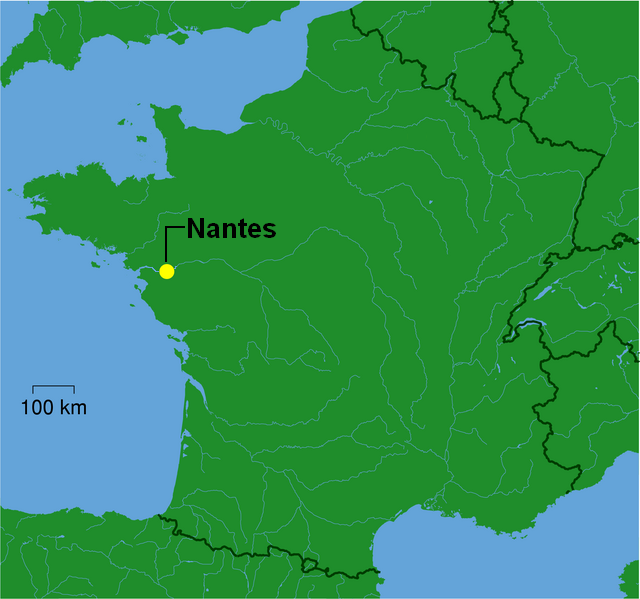
\includegraphics[width=.9\textwidth]{figures/Nantes.png}
\end{center}
\end{column}
\begin{column}{.45\textwidth}
\begin{center}
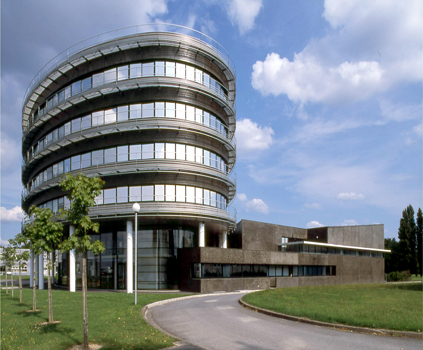
\includegraphics[height=.4\textheight]{figures/irccyn.jpg}\\~\\
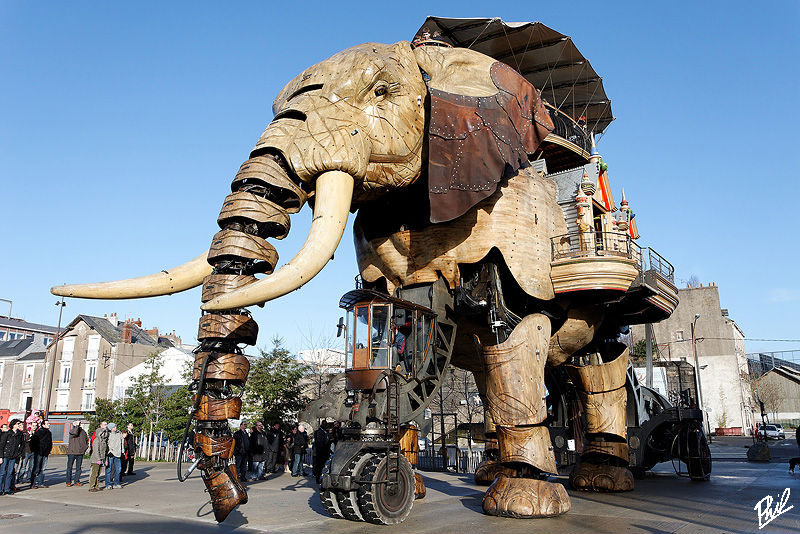
\includegraphics[height=.3\textheight]{figures/machines.jpg}
\end{center}
\end{column}
\end{columns}
\end{frame}

\begin{frame}[c]
  \frametitle{\textbf{MeForBio} (IRCCyN team, ECN)}

%\textbf{MeForBio} (IRCCyN team, ECN): Formal Methods for Bioinformatics

\bigskip\footnotesize
\begin{tabular}{ccc}
  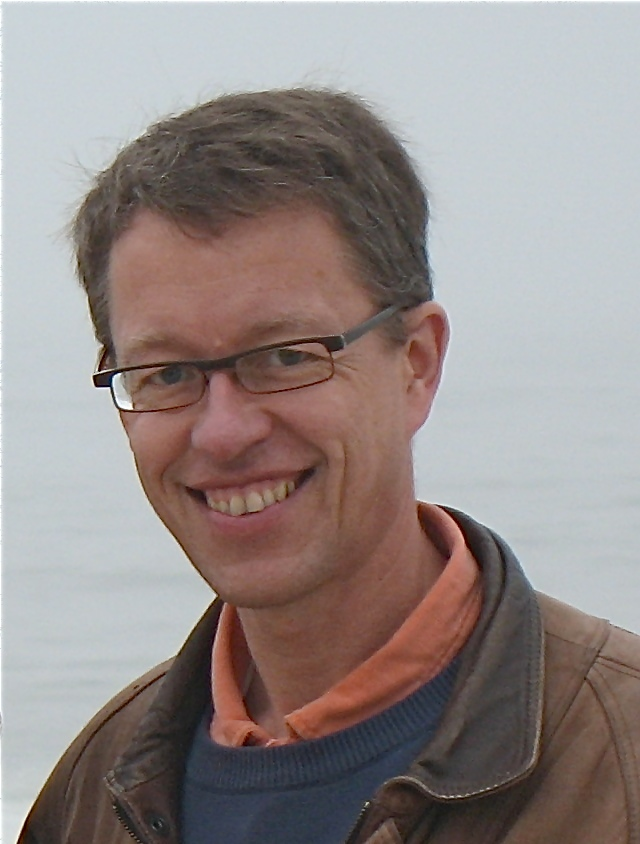
\includegraphics[height=1.5cm]{figures/Olivier.jpg}
& 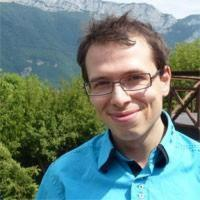
\includegraphics[height=1.5cm]{figures/Morgan.jpg}
& 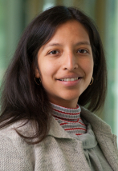
\includegraphics[height=1.5cm]{figures/Carito.jpg} \\
  \tval{Olivier ROUX} & \tval{Morgan MAGNIN} & \tval{Carito GUZIOLOWSKI} \\
  Professor \& team leader & Associate professor & Associate professor \\&&\\
  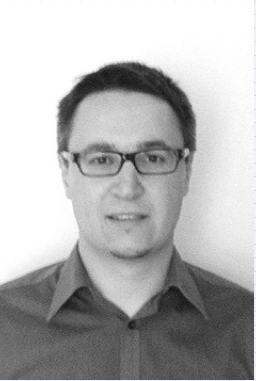
\includegraphics[height=1.5cm]{figures/Julien.jpg}
& 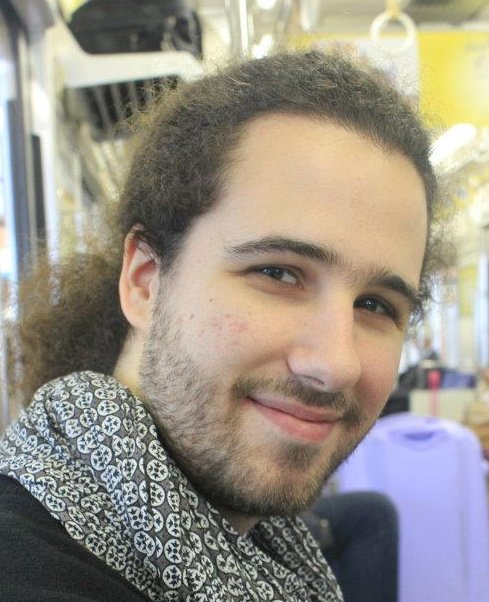
\includegraphics[height=1.5cm]{figures/Maxime.jpg}
& 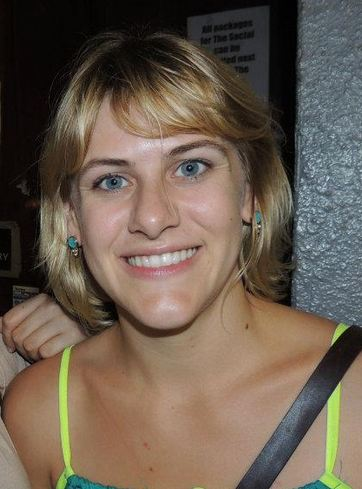
\includegraphics[height=1.5cm]{figures/Courtney.jpg} \\
  \tval{Louis FIPPO FITIME} & \tval{Maxime FOLSCHETTE} & \tval{Courtney CHANCELLOR} \\
  1\textsuperscript{st} year PhD student & 3\textsuperscript{rd} year PhD student & 2\textsuperscript{nd} year PhD student \\    
\end{tabular}
\end{frame}

\frame{\frametitle{\textbf{MeForBio} (IRCCyN team, ECN): Formal Methods for Bioinformatics}

\begin{block}{Research axes}
\begin{itemize}
\item Models: automata, Petri nets, boolean networks, process algebra ($\rightarrow$~process hitting)
\item Extended with: time (\textbf{chronometry} vs \textbf{chronology}) and/or parameters
\item Analysis techniques: \textbf{model-checking}, \textbf{control}, \textbf{abstraction}, \textbf{parameters inference}
\item Applied (and/or designed) to biology, e.g. biological regulatory networks
\end{itemize}
\end{block}

}


\frame{\frametitle{Today's issue}

\begin{alertblock}{Tricky question}
How can we study complex dynamical biological systems, \textbf{involving up to 1.000 interacting components}?
%\begin{center}
%  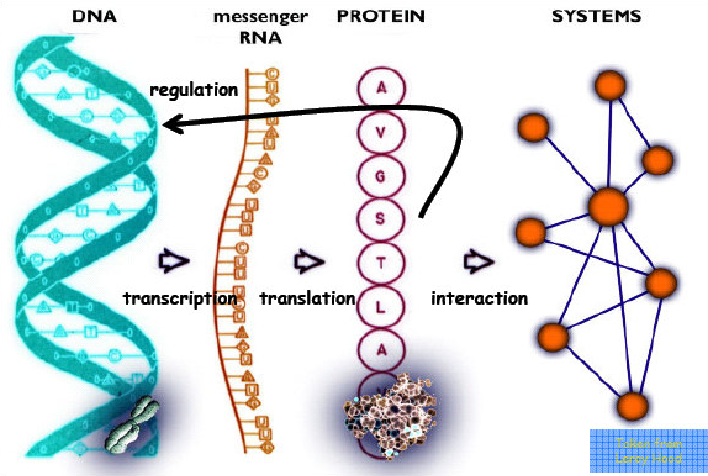
\includegraphics[height=2cm]{figures/dnascheme_white.png}
%\end{center}
\end{alertblock}

\begin{block}{Observation}
\begin{itemize}
\item Classical model-checking approaches suffer from state space explosion
\item Leads:
\begin{itemize}
\item Taking profit for Process Algebra structure, based on a \textbf{compact representation of the interactions} 
\item Develop \textbf{static analysis approaches} to verify some crucial properties, e.g. stable states, reachability, key processes, $\ldots$
\end{itemize}
\end{itemize}
\end{block}

}


\frame{\frametitle{Contribution}

\begin{alertblock}{Scientific challenge}
How can we cope with the analysis of \textbf{large-scale systems}, involving up to 1.000 interacting components?
\end{alertblock}

\begin{block}{Objectives of this talk}
\begin{itemize}
\item Introduce a Process Algebra inspired framework based on a compact representation of the interactions
\item Develop efficient \textbf{static analysis approaches} to answer most common problems 
\item Apply the methodology to large-scale biological regulatory networks 
\end{itemize}
\end{block}

%\begin{block}{Joint work with}
%\begin{itemize}
%\item K. Inoue (NII) 
%\item L. Paulev� (LRI)
%\item O. Roux (IRCCyN) 
%\end{itemize}
%\end{block}

}


\section{Modeling biological regulatory networks: Thomas' framework}
% Définition du modèle de Thomas

\frame{\frametitle{Short introduction to Biological Regulatory Networks}

\begin{block}{Principle of R. Thomas' discrete modeling \cite{thomas1976ac}}
\begin{itemize}
\item \textbf{Activations} and \textbf{inhibitions} between genes
\item Gene/protein couples
\item Genes expression is associated to a set of \texthl{discrete logic} levels
\item \textbf{Effective control} beyond a given \texthl{threshold}; opposite effect below.
\end{itemize}
\end{block}

\begin{block}{Interaction graph} 
\vspace{-1.8em}

\begin{columns}
\begin{column}{0.5\textwidth}

\medskip
\begin{itemize}
  \item Nodes = \textbf{Genes}
  \item Directed edges = \textbf{Interactions}
  \item But what is the \textbf{evolutionary tendency} of $a$ when $a$ is at level $1$ and $b$ at level $1$? $\Rightarrow$ Need for \alert{\textbf{parametrization}}  %discrete parameters defining the strength of the interactions, based on the set of resources $\Rightarrow$ \textbf{Parametrization}  
\end{itemize}

\end{column}
\begin{column}{0.5\textwidth}

\begin{flushright}
\scalebox{1.2}{
\begin{tikzpicture}[grn,node distance=2cm]
\path[use as bounding box] (-0.6,-1) rectangle (2.3,0.5);
\node(a) {a};
\node(b) [right of=a] {b};
\path
  (a) edge[inh, bend left] node[elabel, above] {$2-$} (b)
  (b) edge[inh, bend left] node[elabel, below=-2pt] {$1-$} (a)
  (a) edge[act,loop left=10] node[elabel, left] {$1+$} (a);
\path
  node[elabel, below=-1em of a] {$0..2$}
  node[elabel, below=-10pt of b] {$0..1$};
%\node (ba) [elabel,below of=a,below=-2pt] {$0..2$} (a);
%\node (bb) [elabel,below of=b] {$0..1$};
\end{tikzpicture}
}
%
%+ Parametrization \quad~
\end{flushright}

\end{column}
\end{columns}

\end{block}
}

\begin{frame}
  \frametitle{Biological Regulatory Network (Thomas' modeling)}
%  \framesubtitle{\tcite{RCB08}}

~~~\begin{tabular}{cccc}
%
\begin{tikzpicture}[grn]
\path[use as bounding box] (-0.7,-0.3) rectangle (2.5,2);
% Nœuds noirs
\only<1,3->{
  \node[inner sep=0] (z) at (2,0.75) {z};
  \node[inner sep=0] (a) at (0,1.5) {a};
  \node[inner sep=0] (b) at (0,0) {b};
  \path
    node[elabel, below=-1em of a] {$0..1$}
    node[elabel, below=-1em of b] {$0..1$}
    node[elabel, below=-1em of z] {$0..2$};
}
% Nœuds grisés
\only<2>{
  \node[inner sep=0,light] (z) at (2,0.75) {z};
  \node[inner sep=0,light] (a) at (0,1.5) {a};
  \node[inner sep=0,light] (b) at (0,0) {b};
  \path
    node[elabel, below=-1em of a,light] {$0..1$}
    node[elabel, below=-1em of b,light] {$0..1$}
    node[elabel, below=-1em of z,light] {$0..2$};}

%% Arcs colorés
\only<1,4->{\path
  (a) edge[inh,loop left=10] node[elabel, left] {$1-$} (a)
  (a) edge[act] node[elabel, above=-2pt] {$1+$} (z)
  (b) edge[inh] node[elabel, below=-2pt] {$1-$} (z);}
% Arcs grisés
\only<2-3>{\path
  (a) edge[inhgray,loop left=10] node[elabel, left,light] {$1-$} (a)
  (a) edge[actgray] node[elabel, above=-2pt,light] {$1+$} (z)
  (b) edge[inhgray] node[elabel, below=-2pt,light] {$1-$} (z);
}
\end{tikzpicture}
&%
\only<2-4>{\color{light}}
\begin{tabular}[b]{c|c|c}
  \multicolumn{2}{c|}{$\omega$} & \multirow{2}{*}{$k_{z, \omega}$} \\
\cline{1-2}
  $a$ & $b$ & \\
\hline
  $-$ & $+$ & $1$ \\
  $-$ & $-$ & $0$ \\
  \only<6>{\color{red}}$+$ & \only<6>{\color{red}}$+$ & \only<6>{\color{red}}$2$ \\
  $+$ & $-$ & $1$
\end{tabular}
%%\begin{tabular}[b]{c|c}
%%  $\omega$ & $k_{z, \omega}$ \\
%%\hline
%%  $\emptyset$ & $1$ \\
%%  $\{b\}$ & $0$ \\
%%  \only<7-8>{\color{red}}$\{a\}$ & \only<7-8>{\color{red}}$2$ \\
%%  $\{a;b\}$ & $1$
%%\end{tabular}
~~~~&
\only<2-4>{\color{light}}%
\begin{tabular}[b]{c|c}
  $\omega$ & \multirow{2}{*}{$k_{a, \omega}$} \\
\cline{1-1}
  $a$ & \\
\hline
  $+$ & $1$ \\
  $-$ & $0$
\end{tabular}
%%\begin{tabular}[b]{c|c}
%%  $\omega$ & $k_{a, \omega}$ \\
%%\hline
%%  $\emptyset$ & $1$ \\
%%  $\{a\}$ & $0$
%%\end{tabular}
&
\only<2-4>{\color{light}}%
\begin{tabular}[b]{cc}
  & $k_{b, \omega}$ \\
\cline{2-2}
  & $1$
\end{tabular}
%%\begin{tabular}[b]{c|c}
%%  $\omega$ & $k_{b, \omega}$ \\
%%\hline
%%  $\emptyset$ & $1$
%%\end{tabular}
\\
\only<2-4>{$\underbrace{\text{~\hspace{3cm}~}}_{\text{Interaction Graph}}$}%
&
\multicolumn{3}{r}{\only<5->{$\underbrace{\text{~\hspace{6.5cm}~}}_\text{Parametrization}$}}
\end{tabular}

\bigskip
% Historical model...
\only<1>{

\bigskip
Proposed by Ren\'e Thomas in 1973, several extensions since then
\medskip
\begin{liste}
  \item \tval{Historical bio-informatics model} for studying genes interactions
  \item Widely used and well-adapted to represent dynamic gene systems
\end{liste}
}

% Interaction Graph
\only<2-4>{
\tval{Interaction Graph}: structure of the system (genes \& interactions)

\pause[3]
\medskip
\begin{liste}
  \item \tval{Nodes}: genes
  \begin{itemize}
    \item Name \qex{$a$, $b$, $z$}
    \item Possible values (levels of expression) \qex{$0..1$, $0..2$}
  \end{itemize}
\pause[4]
  \item \tval{Edges}: interactions
  \begin{itemize}
    \item Threshold \qex{$1$}
    \item Type (activation or inhibition) \qex{$+$ / $-$}
  \end{itemize}
\end{liste}
}

% Parametrization
\only<5->{
\medskip
\tval{Parametrization}: strength of the influences (cooperations)

\medskip
\begin{liste}
  \item Maps of tendencies for each gene
  \begin{fleches}
    \item To any \tval{influences of predecessors} \qex{$\omega$}
    \item Corresponds a \tval{parameter} \qex{$k_{x,\omega}$}
  \end{fleches}
\pause[6]
\medskip
  \item \ex{$k_{z, \{a^+, b^+\}} = 2$} \quad means: \qex{$z$ tends to $2$ when $a \geq 1$ and $b < 1$}
\end{liste}
%\pause[10]
}
\end{frame}



\begin{frame}
  \frametitle{Biological Regulatory Network (Thomas' modeling)}
%  \framesubtitle{\tcite{RCB08}}

\begin{tabular}{cccc}

~~~\begin{tikzpicture}[grn]
\path[use as bounding box] (-0.7,-0.3) rectangle (2.5,2);
\node[inner sep=0] (z) at (2,0.75) {z};
\node[inner sep=0] (a) at (0,1.5) {a};
\node[inner sep=0] (b) at (0,0) {b};
\path
  node[elabel, below=-1em of a] {$0..1$}
  node[elabel, below=-1em of b] {$0..1$}
  node[elabel, below=-1em of z] {$0..2$};
\path
  (a) edge[inh,loop left=10] node[elabel, left] {$1-$} (a)
  (a) edge[act] node[elabel, above=-2pt] {$1+$} (z)
  (b) edge[inh] node[elabel, below=-2pt] {$1-$} (z);
\end{tikzpicture}
&
\begin{tabular}[b]{c|c|c}
  \multicolumn{2}{c|}{$\omega$} & \multirow{2}{*}{$k_{z, \omega}$} \\
\cline{1-2}
  $a$ & $b$ & \\
\hline
  $-$ & $+$ & $1$ \\
  $-$ & $-$ & $0$ \\
  $+$ & $+$ & $2$ \\
  $+$ & $-$ & $1$
\end{tabular}
~~~~&
\begin{tabular}[b]{c|c}
  $\omega$ & \multirow{2}{*}{$k_{a, \omega}$} \\
\cline{1-1}
  $a$ & \\
\hline
  $+$ & $1$ \\
  $-$ & $0$
\end{tabular}
&
\begin{tabular}[b]{cc}
   & $k_{b, \omega}$ \\
\cline{2-2}
   & $1$
\end{tabular}
\\
\multicolumn{4}{r}{$\underbrace{\text{\hspace{10.1cm}}}_{\text{Biological Regulatory Network}}$}
\end{tabular}

\bigskip

\begin{itemize}
  \item[\f] All needed information to run the model or study its dynamics:
  \begin{itemize}\normalsize
    \item Build the State Graph
    \item Find reachability properties, fixed points, attractors
    \item Other properties...
  \end{itemize}
\end{itemize}

\begin{itemize}
  \item[\f] \tval{Strengths}: well adapted for the study of biological systems
  \item[\f] \tval{Drawbacks}: inherent complexity; needs the full\\
    \quad \quad specification of cooperations
\end{itemize}
\end{frame}


\section[Process Hitting]{The Process Hitting: a framework well suited to concurrent systems}
\subsection{Definition}
% Exemples

% Exemple des définitions + points fixes
\def \exdef {
\TSort{(0,0)}{z}{3}{l}
\TSort{(3,3)}{b}{2}{t}
\TSort{(6,0)}{a}{2}{r}

\THit{b_0}{}{z_1}{.east}{z_2}
\THit{b_1}{}{z_0}{.east}{z_2}
\THit{a_0}{}{b_1}{.south}{b_0}
\THit{a_1}{out=60,in=0,selfhit}{a_1}{.east}{a_0}

\path[bounce,bend right]
\TBounce{z_1}{}{z_2}{.south}
\TBounce{z_0}{bend right=50}{z_2}{.south east}
;
\path[bounce,bend left]
\TBounce{a_1}{}{a_0}{.north}
\TBounce{b_1}{}{b_0}{.south}
;
}

% Idem réorganisé pour Points Fixes
\def \exdefb {
\path[use as bounding box] (0,-1) rectangle (4,4);

\TSort{(0,0)}{z}{3}{l}
\TSort{(2,4)}{b}{2}{t}
\TSort{(4,1)}{a}{2}{r}
}

% Frappes
\def \exdefbfrappes {
\THit{b_0}{}{z_1}{.east}{z_2}
\THit{b_1}{}{z_0}{.east}{z_2}
\THit{a_0}{}{b_1}{.south}{b_0}
\THit{a_1}{out=60,in=0,selfhit}{a_1}{.east}{a_0}

\path[bounce,bend right]
\TBounce{z_1}{}{z_2}{.south}
\TBounce{z_0}{bend right=50}{z_2}{.south east}
;
\path[bounce,bend left]
\TBounce{a_1}{}{a_0}{.north}
\TBounce{b_1}{}{b_0}{.south}
;
}

% Non-frappes
\def \exdefbsf {
\path[use as bounding box] (0,-1) rectangle (4,4);
\node[process,draw=red,thick] (a_1) at (a_1.center) {};

\path<2,4-> (z_0) edge (b_0) edge (a_0) (b_0) edge (a_0);
\path<2-3> (z_2) edge (b_0) edge (a_0);
\path<3>[very thick] (z_0) edge (b_0) edge (a_0) (b_0) edge (a_0);
\path<4->[very thick] (z_2) edge (b_0) edge (a_0) (b_0) edge (a_0);
\TState{3}{z_0,b_0,a_0}
\TState{4-}{z_2,b_0,a_0}

\path (z_2) edge (b_1);
\path (z_1) edge (b_1);
\path (z_1) edge (a_0);
}



% Figure de présentation de l'analyse d'atteignabilité
\def \figsa {
\begin{tikzpicture}
\path[use as bounding box] (-5,-2.6) rectangle (5,2.8);
\definecolor{r2}{RGB}{238,10,38}

\path<2->[shading=1, inner color=r2, outer color=white] (3.5,-2.8) -- (4.4,3.2) -- (0,3) -- (-4.5,1.4) -- (-2.5,-2.5) -- (0,-3.6) -- (2.8,-2.8);
%\path<2->[shading, inner color=r2, outer color=white, border color=white] (2.8,-2.8) -- (4.5,4.5) -- (0,3.9) -- (-4.5,1.8) -- (-5,-3) -- (0,-3.2) -- (2.8,-2.8);
\draw<2->[thick,fill=white] (2.5,-2.1) -- (3,2.5) -- (-2.7,1.3) -- (-2,-2) -- (2.5,-2.1);
\draw<6->[thick,fill=lightyellow] (2.5,-2.1) -- (3,2.5) -- (-2.7,1.3) -- (-2,-2) -- (2.5,-2.1);

\node<2->[text width=3.5cm, color=red] (s1) at (-5,2) {Over-Approximation};
\path<2->[->,very thick,color=red] (s1.south) edge (-3.5,1.2);
%\node<2->[text width=3cm,color=black] (i1) at (3.7,.2) {$\Rightarrow$};
\node<2->[text width=3cm,color=black] (q) at (4.5,.2) {$\neg Q$};

\draw<4->[thick, fill=green] (.5,-.8) -- (1,0) -- (.3,1) -- (-1,.5) -- (-.5,-.5) -- (.5,-.8);
\node<4->[text width=3.5cm,color=darkgreen] (s2) at (5.2,-1.5) {Under-Approximation};
\node<4->[text width=3cm,color=black] (p) at (1.8,.2) {$P$};
%\node<4->[text width=3cm,color=black] (i1) at (2.25,.2) {$\Rightarrow$};

% reaching set
\node[text width=3cm,color=darkcyan] (s) at (1.8,1.7) {Exact solution};
\node<1->[text width=3cm,color=darkcyan] (s0) at (0,0) {};
\draw[color=darkcyan, thick] (0,0) ellipse (2 and 1.5);
%\path<1>[draw=white] (2.8,-2.8) -- (4.5,4.5) -- (0,3.9) -- (-4.5,1.8) -- (-5,-3) -- (-2.5,-3.5) -- (0,-3.2) -- (2.8,-2.8);
\node[text width=3cm,color=black] (r) at (2.8,.2) {$R$};

\path<4->[->,very thick,color=darkgreen] (s2) edge (.6,-.4);

\tikzstyle{point}=[circle,draw=blue,fill=blue,minimum size=5pt,inner sep=0pt]

%\only<5->{
\only<3->{
\node[point] at (-2.4,-2) {};
\node[point] at (-2,2) {};
}
\only<5->{
\node[point] at (0,0) {};
}
\only<7->{
\node[point] at (-.5,-1.1) {};
\node[point] at (2.5,1) {};
}
%}

\end{tikzpicture}
}



% Exemple atteignabilité
\def \exatt {
\path[use as bounding box] (-1,-3) rectangle (7,2);
\TSort{(0,0)}{a}{2}{l}
\TSort{(3,0)}{b}{3}{l}
\TSort{(6,0)}{d}{3}{r}
\TSort{(2,-2)}{c}{2}{b}

\THit{a_0}{}{c_0}{.north}{c_1}
\THit{a_1}{}{b_1}{.west}{b_0}
\THit{c_1}{bend left=20pt}{b_0}{.west}{b_1}
\THit{b_1.south west}{->}{a_0}{.east}{a_1}
\THit{b_0}{}{d_0}{.west}{d_1}
\THit{b_1}{}{d_1}{.west}{d_2}
\THit{d_1}{}{b_0}{.north east}{b_2}
\THit{c_1}{bend right=80pt,distance=80pt}{d_1}{.east}{d_0}
\THit{b_2}{distance=120pt,out=30,in=40}{d_0}{.east}{d_2}

\path[bounce,bend left]
\TBounce{d_0}{}{d_1}{.south}
\TBounce{d_1}{}{d_2}{.south}
\TBounce{c_0}{}{c_1}{.west}
\TBounce{b_0}{}{b_1}{.south}
\TBounce{d_1}{}{d_0}{.north}
;
\path[bounce,bend right]
\TBounce{a_0}{}{a_1}{.south}
\TBounce{b_0}{}{b_2}{.south}
\TBounce{b_1}{}{b_0}{.north}
\TBounce{d_0}{bend right=50pt,distance=40pt}{d_2}{.south}
;
}



% Structure abstraite / Sous-approximation / Ok
\def \sauyes {%
\begin{tikzpicture}[aS,node distance=1.1cm,shorthandon]
\path[use as bounding box] (-0.5,-2.1) rectangle (10.25,2.2);

\node[Aobj] (d02) {$\PHobjectif{d_0}{d_2}$};
\node[Aproc,above of=d02] (d2) {$d_2$};

\node[Asol,right of=d02] (d02s2) {};
\node[Aproc,above right of=d02s2] (b0) {$b_0$};
\node[Aobj,right of=b0] (b10) {$\PHobjectif{b_1}{b_0}$};
\node[Asol,right of=b10] (b10s) {};
\node[Aproc,right of=b10s] (a1) {$a_1$};
\node[Aobj,right of=a1] (a11) {$\PHobjectif{a_1}{a_1}$};
\node[Asol,right of=a11] (a11s) {};

\node[Aobj,above of=b10,yshift=-0.5cm] (b00)
{$\PHobjectif{b_0}{b_0}$};
\node[Asol,right of=b00] (b00s) {};

\node[Aproc, below of=b0] (b1) {$b_1$};
\node[Aobj,right of=b1] (b11) {$\PHobjectif{b_1}{b_1}$};
\node[Asol,right of=b11] (b11s) {};
\node[Aobj,below of=b11] (b01) {$\PHobjectif{b_0}{b_1}$};
\node[Asol,right of=b01] (b01s) {};
\node[Aproc,right of=b01s] (c1) {$c_1$};
\node[Aobj,right of=c1] (c11) {$\PHobjectif{c_1}{c_1}$};
\node[Asol,right of=c11] (c11s) {};

\path
(d02) edge (d02s2) (d02s2) edge (b1) edge (b0)
(a11) edge (a11s)
(b10) edge (b10s) (b10s) edge (a1)
(b11) edge (b11s)
(b0) edge (b10) (b1) edge (b11)
(a1) edge (a11)
(d2) edge (d02)
;
\path
(b0) edge (b00.west) (b00) edge (b00s)
(b1) edge (b01)
(b01) edge (b01s) (b01s) edge (c1)
(c1) edge (c11) (c11) edge (c11s)
;
%\node<\tu>[right of=a11s] {\textbf{\Large\color{darkgreen}Yes}};
\end{tikzpicture}%
}

% Structure abstraite / Sous-approximation / Inconclusif
\def \sauinconc {%
\begin{tikzpicture}[aS,node distance=1.1cm,shorthandon]
\path[use as bounding box] (-0.5,-2.1) rectangle (10.25,2.2);

\node[Aobj] (d02) {$\PHobjectif{d_0}{d_2}$};
\node[Aproc,above of=d02] (d2) {$d_2$};

\node[Asol,right of=d02] (d02s2) {};
\node[Aproc,above right of=d02s2] (b0) {$b_0$};
\node[Aobj,right of=b0] (b10) {$\PHobjectif{b_1}{b_0}$};
\node[Asol,right of=b10] (b10s) {};
\node[Aproc,right of=b10s] (a1) {$a_1$};
\node[Aobj,right of=a1] (a01) {$\PHobjectif{a_0}{a_1}$};
\node[Asol,right of=a01] (a01s) {};

\node[Aproc, below of=b0] (b1) {$b_1$};
\node[Aobj,right of=b1] (b11) {$\PHobjectif{b_1}{b_1}$};
\node[Asol,right of=b11] (b11s) {};
\node[Aobj,below of=b11] (b01) {$\PHobjectif{b_0}{b_1}$};
\node[Asol,right of=b01] (b01s) {};
\node[Aproc,right of=b01s] (c1) {$c_1$};
\node[Aobj,right of=c1] (c01) {$\PHobjectif{c_0}{c_1}$};
\node[Asol,right of=c01] (c01s) {};
\node[Aproc,right of=c01s] (a0) {$a_0$};
\node[Aobj,right of=a0] (a00) {$\PHobjectif{a_0}{a_0}$};
\node[Asol,right of=a00] (a00s) {};

\node[Aobj,above of=b10] (b00) {$\obj{b_0}{b_0}$};
\node[Asol,right of=b00] (b00s) {};
\node[Aobj,above of=a01] (a11) {$\obj{a_1}{a_1}$};
\node[Asol,right of=a11] (a11s) {};
\node[Aobj,above of=c01] (c11) {$\obj{c_1}{c_1}$};
\node[Asol,right of=c11] (c11s) {};
\node[Aobj,above of=a00] (a10) {$\PHobjectif{a_1}{a_0}$};
\node at (a10.east) {\Large\color{red}\textbf{$\bot$}};

\path
  (b10) edge[loop,min distance=5mm] (b10)
 ;
\path
(d02) edge (d02s2) (d02s2) edge (b1) edge (b0)
(a01) edge (a01s) (a01s.south) edge (b1.north east)
(b10) edge (b10s) (b10s) edge (a1)
(b11) edge (b11s)
(a1) edge (a01)
(b0) edge (b10) (b1) edge (b11)
(d2) edge (d02)
;
\path
(b00) edge (b00s)
(b0) edge (b00)
 (b1) edge (b01)
 (b01) edge (b01s) (b01s) edge (c1)
 (c1) edge (c01)
 (c01) edge (c01s) (c01s) edge (a0)
 (a0) edge (a00) (a00) edge (a00s)
;
\path
 (c1) edge (c11) (c11) edge (c11s)
(a0) edge (a10)
(a1) edge (a11)
(a11) edge (a11s)
;

%\node[right of=a01s] {\textbf{\Large\color{darkyellow}Inconc}};

\end{tikzpicture}%
}

% Structure abstraite / Sur-approximation / Non
\def \saono {%
\begin{tikzpicture}[aS,node distance=1.1cm,shorthandon]
\path[use as bounding box] (-0.5,-2.1) rectangle (10.25,1.15);

\node[Aobj] (d12) {$\PHobjectif{d_1}{d_2}$};
\node[Asol,above right of=d12] (d12s1) {};
\node[Aproc, right of=d12s1] (b2) {$b_2$};
\node[Aobj,right of=b2] (b02) {$\PHobjectif{b_0}{b_2}$};
\node[Asol,right of=b02] (b02s) {};
\node[Aproc,right of=b02s] (d1) {$d_1$};
\node[Aobj,right of=d1] (d11) {$\PHobjectif{d_1}{d_1}$};
\node[Asol,right of=d11] (d11s) {};

\node[Asol,below right of=d12] (d12s2) {};
\node[Aproc, right of=d12s2] (b1) {$b_1$};
\node[Aobj,right of=b1] (b01) {$\PHobjectif{b_0}{b_1}$};
\node[Asol,right of=b01] (b01s) {};
\node[Aproc,right of=b01s] (c1) {$c_1$};
\node[Aobj,right of=c1] (c01) {$\PHobjectif{c_0}{c_1}$};
\node[Asol,right of=c01] (c01s) {};
\node[Aproc,right of=c01s] (a0) {$a_0$};
\node[Aobj,right of=a0] (a10) {$\PHobjectif{a_1}{a_0}$};
\node at (a10.east) {\Large\color{red}\textbf{$\bot$}};

\path
(d12) edge (d12s1) edge (d12s2) (d12s1) edge (b2) edge (c1) (d12s2) edge (b1)
(b01) edge (b01s) (b01s) edge (c1)
(b02) edge (b02s) (b02s) edge (d1)
(c01) edge (c01s) (c01s) edge (a0)
(d11) edge (d11s)
(a0) edge (a10)
(b1) edge (b01)
(b2) edge (b02)
(c1) edge (c01)
(d1) edge (d11)
;
%\only<\value{anim1}>{ \node[above right of=c01s] {\textbf{\Large\color{red}No}};}
\end{tikzpicture}%
}

% Structure abstraite / Sur-approximation / Inconclusif
\def \saoinconc {%
\begin{tikzpicture}[aS,node distance=1.1cm,shorthandon]
\path[use as bounding box] (-0.5,-2.1) rectangle (10.25,1.15);

\node[Aobj] (d02) {$\PHobjectif{d_0}{d_2}$};
\node[Asol,above right of=d02] (d02s1) {};

\node[Aproc, right of=d02s1] (b2) {$b_2$};
\node[Aobj,right of=b2] (b12) {$\PHobjectif{b_1}{b_2}$};
\node[Asol,right of=b12] (b12s) {};
\node[Aproc,right of=b12s] (d1) {$d_1$};
\node[Aobj,right of=d1] (d01) {$\PHobjectif{d_0}{d_1}$};
\node[Asol,right of=d01] (d01s) {};

\node[Asol,below right of=d02] (d02s2) {};
%<-3>
\node<-\tof>[Aproc, right of=d02s2] (b0) {$b_0$};
\node<\tokp>[orange, thick, Aproc, right of=d02s2] (b0) {$b_0$};
\node[Aobj,right of=b0] (b10) {$\PHobjectif{b_1}{b_0}$};
\node[Asol,right of=b10] (b10s) {};
%<-3>
\node<-\tof>[Aproc,right of=b10s] (a1) {$a_1$};
\node<\tokp>[orange, thick, Aproc,right of=b10s] (a1) {$a_1$};
\node[Aobj,right of=a1] (a11) {$\PHobjectif{a_1}{a_1}$};
\node[Asol,right of=a11] (a11s) {};

\node[Aproc, below of=b0] (b1) {$b_1$};
\node[Aobj,right of=b1] (b11) {$\PHobjectif{b_1}{b_1}$};
\node[Asol,right of=b11] (b11s) {};

\node<\tokp>[orange, font=\bfseries,below of=a11s] (kp) {Key processes};
\path<\tokp>[orange, thick]
        (kp) edge (a1)
        (kp) edge (b0)
;
\path
(d02) edge (d02s1) edge (d02s2) (d02s1) edge (b2) (d02s2) edge (b1) edge (b0)
(a11) edge (a11s)
(b10) edge (b10s) (b10s) edge (a1)
(b11) edge (b11s)
(b12) edge (b12s) (b12s) edge (d1) edge (a1)
(d01) edge (d01s) (d01s.south) edge (b0)
(a1) edge (a11)
(b0) edge (b10) (b1) edge (b11) (b2) edge (b12)
(d1) edge (d01)
;
%\node[below right of=d01s] {\textbf{\Large\color{yellow}Inconc}};
\end{tikzpicture}%
}

%\frame{\frametitle{Contribution}
%
%\begin{alertblock}{Scientific challenge}
%How can we cope with the analysis of \textbf{large-scale systems}, involving up to 1.000 interacting components?
%\end{alertblock}
%
%\begin{block}{Objectives of this part}
%\begin{itemize}
%\item Introduce a Process Algebra inspired framework based on a compact representation of the interactions
%\item Develop efficient \textbf{static analysis approaches} to answer most common problems 
%\item Apply the methodology to large-scale biological regulatory networks 
%\end{itemize}
%\end{block}
%
%\begin{block}{Joint work with}
%\begin{itemize}
%\item L. Paulev� (ETH Zurich), M. Folschette, O. Roux (IRCCyN) 
%\item K. Inoue (NII) 
%\end{itemize}
%\end{block}
%
%}

% Définition du Process Hitting + sortes coopératives

\frame{\frametitle{Intuitive principle of the Process Hitting framework}

\begin{center}
\begin{tabular}{l l p{70mm}}
Process & = & component \texthl{$a$} at level \texthl{$i$}\\
Interaction & = & \texthl{$a$} at level \texthl{$i$} makes \texthl{$b$} at level \texthl{$j$} increase or decrease to level \texthl{$k$}\\
denoted & & \texthl{$\hit{a_i}{b_j}{b_k}$} (hit and bounce)\\
\hline
\end{tabular}

\vfill
{
\begin{definition}[Interaction and Retroaction]\label{def:action}
\emph{Interaction} ($\hit{a_i}{b_j}{b_k}$), where $a_i$ is the level of a process $a$ and $b_j\neq b_k$,

\emph{Retroaction} ($\hit{a_i}{a_i}{a_k}$): when $a_i=b_j$.
\end{definition}
}
\end{center}

}

\begin{frame}[t]
  \frametitle{The Process Hitting modeling}
%  \framesubtitle{\cite{PMR10-TCSB}}

% 1 : Sortes
\only<1>{
\tikzstyle{process}=[circle,minimum size=15pt,font=\footnotesize,inner sep=1pt]
\tikzstyle{tick label}=[color=white, font=\footnotesize]
\tikzstyle{tick}=[transparent]
\tikzstyle{hit}=[transparent]
\tikzstyle{selfhit}=[transparent, min distance=30pt,curve to]
\tikzstyle{bounce}=[transparent]
\tikzstyle{hlhit}=[transparent]
\begin{center}\scalebox{\scaleex}{
\begin{tikzpicture}
\exphdef
\end{tikzpicture}
}\end{center}
}

% 2 : Processus
\only<2>{
\tikzstyle{process}=[circle,draw,minimum size=15pt,font=\footnotesize,inner sep=1pt]
\tikzstyle{tick label}=[font=\footnotesize]
\tikzstyle{tick}=[densely dotted]
\tikzstyle{hit}=[transparent]
\tikzstyle{selfhit}=[transparent, min distance=30pt,curve to]
\tikzstyle{bounce}=[transparent]
\tikzstyle{hlhit}=[transparent]
\begin{center}\scalebox{\scaleex}{
\begin{tikzpicture}
\exphdef
\end{tikzpicture}
}\end{center}
}

% 3 : États
\only<3>{
\tikzstyle{hit}=[transparent]
\tikzstyle{selfhit}=[transparent, min distance=30pt,curve to]
\tikzstyle{bounce}=[transparent]
\tikzstyle{hlhit}=[transparent]
\begin{center}\scalebox{\scaleex}{
\begin{tikzpicture}
\exphdef

\TState{3}{a_0,b_1,z_0}
\end{tikzpicture}
}\end{center}
}

% 4 : Actions
\only<4->{
\tikzstyle{tick}=[densely dotted]
\tikzstyle{hit}=[->,>=angle 45]
\tikzstyle{selfhit}=[min distance=30pt,curve to]
\tikzstyle{bounce}=[densely dotted,>=stealth',->]
\tikzstyle{hlhit}=[very thick]
\begin{center}\scalebox{\scaleex}{
\begin{tikzpicture}
\exphdef
\TState{4}{a_0,b_1,z_0}
\TState{5}{a_0,b_1,z_1}
\TState{6}{a_1,b_1,z_1}
\TState{7}{a_1,b_1,z_2}
\end{tikzpicture}
}\end{center}
}

%\smallskip
\vspace*{.18em}
\begin{liste}
  \item \tval{Sorts}: components \qex{$a$, $b$, $z$}
\pause[2]
  \item \tval{Processes}: local states / levels of expression \qex{$z_0$, $z_1$, $z_2$}
\pause[3]
  \item \tval{States}: sets of active processes%
  \only<3-4>{\qex{$\PHetat{a_0, b_1, z_0}$}}%
  \only<5>{\qex{$\PHetat{a_0, b_1, z_1}$}}%
  \only<6>{\qex{$\PHetat{a_1, b_1, z_1}$}}%
  \only<7>{\qex{$\PHetat{a_1, b_1, z_2}$}}%
\pause[4]
  \item \tval{Actions}: dynamics \qex{\only<4>{\underline}{$\PHfrappe{b_1}{z_0}{z_1}$}, \only<4-5>{\underline}{$\PHfrappe{a_0}{a_0}{a_1}$}, \only<6>{\underline}{$\PHfrappe{a_1}{z_1}{z_2}$}}
\end{liste}
\end{frame}



\begin{frame}
  \frametitle{Adding cooperations}
  \framesubtitle{\cite{PMR12-MSCS}}

\begin{center}\scalebox{\scaleex}{
\begin{tikzpicture}
\exphcoop
\end{tikzpicture}
}\end{center}

\medskip
\begin{liste}
  \item How to introduce some \tval{cooperation} between sorts? \qex{$\PHfrappe{\underline{a_1 \wedge b_0}}{z_1}{z_2}$}
\pause[4]
  \item Solution: a \tval{cooperative sort} \qex{$ab$} \pause[12]\quad to express \qex{$\underline{a_1 \wedge b_0}$}
\pause[8]
  \item Constraint: represent each configuration \qex{$\PHetat{\underline{a_1,b_0}} \pause[11]\Rightarrow ab_{10}$}
\pause[14]
  \item Advantage: regular sort; drawbacks: complexity, temporal shift
\end{liste}
\end{frame}



%\subsubsection{Fixed Points}

\begin{frame}[c]
  \frametitle{Static Analysis: Fixed Points}
  \framesubtitle{\cite{PMR10-TCSB}}

\tval{Fixed point} = state where no action can be fired
\begin{fleches}
  \item avoid couples of processes bounded by an action
%\only<1>{\\\smallskip~}
\uncover<2->{\item Hitless Graph} \uncover<3->{\f \tval{n-cliques} = fixed points}
\end{fleches}

\bigskip
\begin{columns}
\begin{column}{0.5\textwidth}

\begin{center}
\scalebox{0.7}{
\begin{tikzpicture}
\exdefb
\exdefbfrappes
\end{tikzpicture}
}
\end{center}

\end{column}
\begin{column}{0.5\textwidth}

\only<2->{
\begin{center}
\scalebox{0.7}{
\tikzstyle{current process}=[process,fill=red]
\begin{tikzpicture}[hitless graph]
\exdefb
\exdefbsf
\end{tikzpicture}
\tikzstyle{current process}=[process,fill=blue]
}
\end{center}
}

\end{column}
\end{columns}

\bigskip
\pause[5]
Exponential complexity w.r.t.~the number of sorts

\end{frame}

%\begin{frame}
%  \frametitle{Static analysis: successive reachability}
%  \framesubtitle{\cite{PMR12-MSCS}}
%  
%  \begin{alertblock}{Problem}
%  Given an initial state of a Process Hitting, is it possible to reach successively $a_i$, then $b_j$, then $a_k$, then $c_l$, $\ldots$? \\
%  $\Rightarrow$ Combinatorial explosion of the dynamics to explore 
%  \end{alertblock}
%  
%  \begin{block}{Key idea}
%  Instead of checking the successive reachability $\mathcal{R}$, which is complex, we will check: 
%  \begin{itemize}
%  \item an \textbf{under-approximation} $\mathcal{P}$: if $\mathcal{P}$ is not satisfied, then $\mathcal{R}$ neither
%  \item an \textbf{over-approximation} $\mathcal{Q}$: if $\mathcal{Q}$ is satisfied, then $\mathcal{R}$ too. 
%  \end{itemize}
%  \end{block}
%  
%\end{frame}  
%%
%\begin{frame}
%  \frametitle{Static analysis: successive reachability}
%  \framesubtitle{\cite{PMR12-MSCS}}
%
%Successive reachability of processes:
%
%\begin{columns}
%\begin{column}{0.55\textwidth}
%
%\begin{center}
%\scalebox{0.75}{
%\begin{tikzpicture}
%%\path[use as bounding box] (-1,-3) rectangle (7,2);
%\exatt
%
%\TState{2-4}{a_0,b_0,b_2,c_0,d_0}
%
%\TState{5}{a_0,b_0,c_0,d_0}
%\TState{6}{a_0,b_0,c_1,d_0}
%\TState{7}{a_0,b_1,c_1,d_0}
%\TState{8}{a_0,b_1,c_1,d_1}
%\TState{9}{a_0,b_1,c_1,d_2}
%
%\node<3>[process,very thick] (d_1) at (d_1.center) {1?};
%\node<3>[process,very thick] (b_1) at (b_1.center) {2?};
%\node<3>[process,very thick] (d_2) at (d_2.center) {3?};
%
%\node<4-8>[process,very thick] (d_2) at (d_2.center) {1?};
%\node<9>[process,very thick] (d_2) at (d_2.center) {};
%
%\only<5>{\THit{a_0}{hlhit}{c_0}{.north}{c_1}}
%\path<5>[bounce,bend left,hlhit] \TBounce{c_0}{}{c_1}{.west};
%\only<6>{\THit{c_1}{bend left=20pt,hlhit}{b_0}{.west}{b_1}}
%\path<6>[bounce,bend left,hlhit] \TBounce{b_0}{}{b_1}{.south};
%\only<7>{\THit{b_0}{hlhit}{d_0}{.west}{d_1}}
%\path<7>[bounce,bend left,hlhit] \TBounce{d_0}{}{d_1}{.south};
%\only<8>{\THit{b_1}{hlhit}{d_1}{.west}{d_2}}
%\path<8>[bounce,bend left,hlhit] \TBounce{d_1}{}{d_2}{.south};
%\end{tikzpicture}
%}
%\end{center}
%
%\end{column}
%\begin{column}{0.45\textwidth}
%
%\pause
%~\\~\\~\\~\\
%\begin{itemize}
%  \item Initial context
%    \\ \rex{\PHetat{a_1, \{b_0, b_1\}, c_0, d_0}} \pause
%  \item Objectives
%    \\ \rex{$[\ \Rsh d_1 \PHconcat\ \Rsh b_1 \PHconcat\ \Rsh d_2\ ]$} \pause
%    \\\smallskip \rex{$[\ \Rsh d_2\ ]$} \pause
%\end{itemize}
%
%\end{column}
%\end{columns}
%
%\medskip
%\begin{center}
%\f Concretization of the objective = scenario
%
%\ex{
%\only<5>{\underline{$\PHfrappe{a_0}{c_0}{c_1}$}}\only<-4,6->{$\PHfrappe{a_0}{c_0}{c_1}$}~\PHconcat~
%\only<6>{\underline{$\PHfrappe{b_0}{d_0}{d_1}$}}\only<-5,7->{$\PHfrappe{b_0}{d_0}{d_1}$}~\PHconcat~
%\only<7>{\underline{$\PHfrappe{c_1}{b_0}{b_1}$}}\only<-6,8->{$\PHfrappe{c_1}{b_0}{b_1}$}~\PHconcat~
%\only<8>{\underline{$\PHfrappe{b_1}{d_1}{d_2}$}}\only<-7,9->{$\PHfrappe{b_1}{d_1}{d_2}$}}
%\end{center}
%
%\end{frame}
%
%
%
%\begin{frame}
%  \frametitle{Over- and Under-approximations}
%  \framesubtitle{\cite{PMR12-MSCS}}
%
%Static analysis by abstractions:
%\begin{fleches}
%  \item Directly checking an objective sequence $R$ is hard
%  \item Rather check the approximations $P$ and $Q$, where \tval{$P \Rightarrow R \Rightarrow Q$}:
%\end{fleches}
%
%\begin{center}
%\scalebox{0.5}{
%\figsa
%}
%\end{center}
%
%\only<-7>{~}
%\only<8->{
%Linear w.r.t.~the number of sorts and \\exponential w.r.t.~the number of processes in each sort
%\begin{fleches}
%  \item Efficient for big models with few levels of expression
%\end{fleches}
%}
%\end{frame}
%
%\begin{frame}
%  \frametitle{Under-approximation}
%
%\def \tu {3}
%\def \tub {4}
%\def \tuf {5}
%
%\begin{columns}
%\begin{column}{0.48\textwidth}
%\begin{center}
%\scalebox{0.55}{
%\begin{tikzpicture}
%\exatt
%\TState{-\tu}{a_1,b_1,c_1,d_0}
%\TState{\tub-}{a_0,b_1,c_0,d_0}
%\node[process,very thick] (d_2) at (d_2.center) {?};
%\end{tikzpicture}
%}
%\end{center}
%
%\end{column}
%\begin{column}{0.52\textwidth}
%
%\f New abstract structure
%
%\tval{Sufficient condition}:
%\smallskip
%
%\only<2->{
%\smallskip
%\begin{itemize}
%  \item \only<-\tu>{no cycle} \only<\tub->{\sout{no cycle}}
%  \item \only<-\tu>{each objective has a solution} \only<\tub->{\sout{each objective has a solution}}
%\end{itemize}
%\begin{center}
%  \only<\tu>{\Large\textcolor{darkgreen}{$R$ is \textbf{true}}} \only<\tuf>{\Large\textcolor{darkyellow}{\textbf{Inconclusive}}}
%\end{center}
%}
%
%\end{column}
%\end{columns}
%
%\only<-\tu>{
%\sauyes
%}
%
%\only<\tub->{
%\sauinconc
%}
%
%\end{frame}
%
%
%
%\begin{frame}
%  \frametitle{Over-approximation}
%
%\def \to {4}
%\def \tob {5}
%\def \tof {6}
%\def \tokp {7}
%
%\begin{columns}
%\begin{column}{0.48\textwidth}
%\begin{center}
%\scalebox{0.55}{
%\begin{tikzpicture}
%\exatt
%\TState{-\to}{a_1,b_0,c_0,d_1}
%\TState{\tob-}{a_1,b_1,c_1,d_0}
%\node[process,very thick] (d_2) at (d_2.center) {?};
%\end{tikzpicture}
%}
%\end{center}
%\bigskip
%
%\end{column}
%\begin{column}{0.52\textwidth}
%
%\tval{Necessary condition}:
%
%\medskip
%\only<2->{
%\only<3-\to>{\sout{There exists a traversal}}\only<2,\tob->{There exists a traversal}
%with no cycle
%
%\smallskip
%\begin{itemize}
%  \item \only<3-\to>{\sout{objective $\rightarrow$ follow one solution}}\only<1-2,\tob->{objective $\rightarrow$ follow one solution}
%  \item solution $\rightarrow$ follow all processes
%  \item process $\rightarrow$ follow all objectives
%\end{itemize}
%\begin{center}
%  \only<\to>{\Large\textcolor{red}{$R$ is \textbf{false}}}\only<\tof->{\Large\textcolor{darkyellow}{\textbf{Inconclusive}}}
%\end{center}
%}
%
%\end{column}
%\end{columns}
%
%%\bigskip
%
%\only<1-\to>{
%\saono
%}
%
%\only<\tob->{
%\saoinconc
%}
%
%\end{frame}
%
%\begin{frame}
%  \frametitle{Stochastic Features}
%  \framesubtitle{\cite{PMR10-TSE}}
%
%\begin{itemize}
%  \item Introduces time features
%  \item Parameters: either $(r,sa)$, or the \tval{firing interval} $[d;D]$.
%\end{itemize}
%
%\begin{columns}
%\begin{column}{0.5\textwidth}
%
%\only<2->{
%\scalebox{0.9}{
%\begin{tikzpicture}[plot,xscale=0.35,yscale=1]
%\draw[axe] (0,0) -- (15.5,0) node[right] {$t$};
%\draw[axe] (0,0) -- (0,1);
%\draw[ticks] (0,0) node[below] {$0$};
%\draw[mean] (4,0) -- (4,0.9) node[right]{$\frac{1}{r}$};
%\draw[dashed] (0.10127,0) -- (0.10127,0.9) node[right] {$d$} (14.75552,0) --
%(14.75552,0.9) node[left] {$D$};
%\pgfplothandlerlineto
%\pgfplotxyfile{plots/BioAtlanSTIC-0409/erlang-0.25-1.table}
%\pgfusepath{stroke}
%\draw[interval] (0.10127,0) -- (14.75552,0);
%\end{tikzpicture}
%}
%
%\scalebox{0.9}{
%\begin{tikzpicture}[plot,xscale=0.35,yscale=1]
%\draw[axe] (0,0) -- (15.5,0) node[right] {$t$};
%\draw[axe] (0,0) -- (0,1);
%\draw[ticks] (0,0) node[below] {$0$};
%\draw[mean] (4,0) -- (4,0.9) node[right]{$\frac{1}{r}$};
%\draw[dashed] (1.29879,0) -- (1.29879,0.9) node[right] {$d$} (8.19327,0) --
%(8.19327,0.9) node[left] {$D$};
%\pgfplothandlerlineto
%\pgfplotxyfile{plots/BioAtlanSTIC-0409/erlang-0.25-5.table}
%\pgfusepath{stroke}
%\draw[interval] (1.29879,0) -- (8.19327,0);
%\end{tikzpicture}
%}
%
%\scalebox{0.9}{
%\begin{tikzpicture}[plot,xscale=0.35,yscale=1]
%\draw[axe] (0,0) -- (15.5,0) node[right] {$t$};
%\draw[axe] (0,0) -- (0,1);
%\draw[ticks] (0,0) node[below] {$0$};
%\draw[mean] (4,0) -- (4,0.9) node[right]{$\frac{1}{r}$};
%\draw[dashed] (2.96888,0) -- (2.96888,0.9) node[left] {$d$} (5.18245,0) --
%(5.18245,0.9) node[right] {$D$};
%\pgfplothandlerlineto
%\pgfplotxyfile{plots/BioAtlanSTIC-0409/erlang-0.25-50.table}
%\pgfusepath{stroke}
%\draw[interval] (2.96888,0) -- (5.18245,0);
%\end{tikzpicture}
%}
%
%~~\textcolor{lightred}{\rule{17mm}{4.5pt}} ~ action duration
%}
%
%\end{column}
%\begin{column}{0.5\textwidth}
%\begin{center}
%
%\only<3->{
%\scalebox{0.9}{
%\begin{tikzpicture}
%\path[use as bounding box] (-1,-1) rectangle (2,1);
%\TSort{(0,0)}{a}{2}{l}
%\TSort{(2,0)}{b}{2}{r}
%\THit{a_0}{}{b_0}{.west}{b_1}
%\THit{a_0}{out=-120,in=180,selfhit}{a_0}{.west}{a_1}
%\path[bounce]
%\TBounce{a_0}{bend left}{a_1}{.south}
%\TBounce{b_0}{bend left}{b_1}{.south}
%;
%\TState{3-}{a_0,b_0}
%\end{tikzpicture}
%}
%
%\scalebox{0.9}{
%\begin{tikzpicture}[plot]
%\node[anchor=west] at (0,0.4) {$\PHfrappe{a_0}{b_0}{b_1}$};
%\draw[axe] (0,0) -- (4,0) node[right] {$t$};
%\draw (0,0.1) -- (0,-0.1);
%\draw[interval] (1.7,0) -- (3,0);
%
%\node[anchor=west] at (0,-0.6) {$\PHfrappe{a_0}{a_0}{a_1}$};
%\draw[axe] (0,-1) -- (4,-1) node[right] {$t$};
%\draw (0,-0.9) -- (0,-1.1);
%\draw[interval,orange] (0.2,-1) -- (1.5,-1);
%\end{tikzpicture}
%}
%
%\noindent
%\f $b_1$ reached with a \tval{very low probability}.
%}
%
%\end{center}
%\end{column}
%\end{columns}
%
%\pause[4]
%\bigskip
%\begin{fleches}
%  \item Tests by \textbf{simulation} and \textbf{model-checking}
%\end{fleches}
%
%\end{frame}
%
%
%


\subsection{From biological models to Process Hitting and refining}
%% Application aux réseaux de régulation biologique
%
%\subsection{Presentation of Interaction Graphs}
%
%\begin{frame}
%  \frametitle{Application to Biological Systems}
%
%\bigskip
%\tval{The Process Hitting framework}:
%\begin{itemize}
%  \item new formalism with simple elements
%  \item dynamic modeling
%  \item efficient reachability checking
%  \item general framework that could be applied to...
%\end{itemize}
%
%\bigskip
%\tval{Biological systems}:
%\begin{itemize}
%  \item gene/protein couples
%  \item Thomas' Modeling: Interaction Graphs
%  \item hard to study \f use Process Hitting
%\end{itemize}
%
%\end{frame}
%
%
%
%\begin{frame}
%  \frametitle{Interaction Graphs}
%
%\begin{columns}
%\begin{column}{0.5\textwidth}
%
%\medskip
%\begin{itemize}
%  \item Nodes = Genes
%  \item Directed edges = Interactions
%\end{itemize}
%
%\end{column}
%\begin{column}{0.5\textwidth}
%
%\begin{flushright}
%\scalebox{1.2}{
%\begin{tikzpicture}[grn,node distance=2cm]
%\path[use as bounding box] (-0.6,-1) rectangle (2.3,0.5);
%\node(a) {a};
%\node(b) [right of=a] {b};
%\path
%  (a) edge[inh, bend left] node[elabel, above] {$-2$} (b)
%  (b) edge[inh, bend left] node[elabel, below=-2pt] {$-1$} (a)
%  (a) edge[act,loop left=10] node[elabel, left] {$+1$} (a);
%\path
%  node[elabel, below=-1em of a] {$0..2$}
%  node[elabel, below=-10pt of b] {$0..1$};
%%\node (ba) [elabel,below of=a,below=-2pt] {$0..2$} (a);
%%\node (bb) [elabel,below of=b] {$0..1$};
%\end{tikzpicture}
%}
%
%+ Parametrization \quad~
%\end{flushright}
%
%\end{column}
%\end{columns}
%
%\bigskip
%
%\only<2>{
%\Large
%\begin{flushright}
%\textcolor{couleurtheme}{State Graphs}\hspace{2em}~\!\!
%\end{flushright}
%\normalsize
%
%\begin{columns}
%\begin{column}{0.4\textwidth}
%
%\begin{itemize}
%  \item One level at a time
%  \item Asynchronous
%\end{itemize}
%
%\end{column}
%\begin{column}{0.6\textwidth}
%
%\begin{flushright}
%\begin{tikzpicture}
%\path[use as bounding box] (0,-2) rectangle (6,-0.5);
%\matrix at (0,0) [anchor=north west,column sep=.8cm, row sep=.8cm]
%{
%\node (s01) {$\PHetat{a_0,b_1}$}; \&
%\node (s11) {$\PHetat{a_1,b_1}$}; \&
%\node (s21) {$\PHetat{a_2,b_1}$}; \\
%\node (s00) {$\PHetat{a_0,b_0}$}; \&
%\node (s10) {$\PHetat{a_1,b_0}$}; \&
%\node (s20) {$\PHetat{a_2,b_0}$}; \\
%};
%\path[->]
%    (s00) edge (s10) edge (s01)
%    (s10) edge (s11) edge (s20)
%    (s21) edge (s11) edge (s20)
%;
%\end{tikzpicture}
%\end{flushright}
%
%\end{column}
%\end{columns}
%
%\bigskip
%Exponential number of states w.r.t.~the number of genes
%}
%\end{frame}
%

%\subsection{Translation from Thomas' framework to Process Hitting \& Refining}

\begin{frame}
  \frametitle{Translation of the Generalized Dynamics}

\begin{center}
Positive interaction:
\end{center}
\begin{columns}
\begin{column}{0.45\textwidth}

\begin{center}
\begin{tikzpicture}[grn,node distance=2cm]
\path[use as bounding box] (-0.8,-.5) rectangle (2.5,0.6);
\node (a) {a};
\node (b) [right of=a] {b};
\path (a) edge[act, bend left] node[elabel, above] {$+1$} (b);
\end{tikzpicture}
\end{center}

\end{column}
\begin{column}{0.05\textwidth}

\begin{flushright}
\medskip
\Large
\f
\normalsize
\end{flushright}

\end{column}
\begin{column}{0.5\textwidth}

\begin{center}
\scalebox{0.8}{
\begin{tikzpicture}
\path[use as bounding box] (-1,0) rectangle (5,1.5);
\TSort{(0,0.5)}{a}{2}{l}
\TSort{(4,0)}{b}{3}{r}

\only<2>{
\THit{a_1}{}{b_0}{.west}{b_1}
\THit{a_1}{}{b_1}{.west}{b_2}
\path[bounce,bend left]
\TBounce{b_0}{}{b_1}{.south west}
\TBounce{b_1}{}{b_2}{.south west};
}

\only<3->{
\THit{a_1}{ulhit}{b_0}{.west}{b_1}
\THit{a_1}{ulhit}{b_1}{.west}{b_2}
\path[bounce,bend left,pulhit]
\TBounce{b_0}{bulhit}{b_1}{.south west}
\TBounce{b_1}{bulhit}{b_2}{.south west};
\THit{a_0}{}{b_2}{.west}{b_1}
\THit{a_0}{}{b_1}{.west}{b_0}
\path[bounce,bend right]
\TBounce{b_2}{}{b_1}{.north west}
\TBounce{b_1}{}{b_0}{.north west};
}

\end{tikzpicture}
}
\end{center}

\end{column}
\end{columns}

\bigskip
\only<4->{
\begin{center}
Negative interaction:
\end{center}
\begin{columns}
\begin{column}{0.45\textwidth}

\begin{center}
\begin{tikzpicture}[grn,node distance=2cm]
\path[use as bounding box] (-0.8,-.5) rectangle (2.5,0.6);
\node (a) {a};
\node (b) [right of=a] {b};
\path (a) edge[inh, bend left] node[elabel, above] {$-1$} (b);
\end{tikzpicture}
\end{center}

\end{column}
\begin{column}{0.05\textwidth}

\begin{flushright}
\medskip
\Large
\f
\normalsize
\end{flushright}

\end{column}
\begin{column}{0.5\textwidth}

\begin{center}
\scalebox{0.8}{
\begin{tikzpicture}
\path[use as bounding box] (-1,0) rectangle (5,1.5);
\TSort{(0,0.5)}{a}{2}{l}
\TSort{(4,0)}{b}{3}{r}

\only<5>{
\THit{a_1}{}{b_2}{.west}{b_1}
\THit{a_1}{}{b_1}{.west}{b_0}
\path[bounce,bend right]
\TBounce{b_2}{}{b_1}{.north west}
\TBounce{b_1}{}{b_0}{.north west};
}

\only<6>{
\THit{a_1}{ulhit}{b_2}{.west}{b_1}
\THit{a_1}{ulhit}{b_1}{.west}{b_0}
\path[bounce,bend right,pulhit]
\TBounce{b_2}{bulhit}{b_1}{.north west}
\TBounce{b_1}{bulhit}{b_0}{.north west};
\THit{a_0}{}{b_0}{.west}{b_1}
\THit{a_0}{}{b_1}{.west}{b_2}
\path[bounce,bend left]
\TBounce{b_0}{}{b_1}{.south west}
\TBounce{b_1}{}{b_2}{.south west};
}

\end{tikzpicture}
}
\end{center}

\end{column}
\end{columns}
}

\end{frame}



%\begin{frame}
%  \frametitle{Refining with Actions Removal}
%
%\bigskip
%Prevent behaviors by deleting \tval{unrealistic actions}
%
%\bigskip
%\begin{center}
%\begin{tikzpicture}
%%\path[use as bounding box] (-1,0) rectangle (5,3);
%\TSort{(0,0.5)}{a}{2}{l}
%\TSort{(4,0)}{b}{3}{r}
%
%\THit{a_0}{ulhit}{b_2}{.west}{b_1}
%\THit{a_0}{ulhit}{b_1}{.west}{b_0}
%\path[bounce,bend right,pulhit]
%\TBounce{b_2}{bulhit}{b_1}{.north west};
%\path[bounce,bend right,pulhit]
%\TBounce{b_1}{bulhit}{b_0}{.north west};
%\THit{a_1}{}{b_0}{.west}{b_1}
%\path[bounce,bend left]
%\TBounce{b_0}{}{b_1}{.south west};
%
%\only<1>{
%\THit{a_1}{}{b_1}{.west}{b_2}
%\path[bounce,bend left]
%\TBounce{b_1}{}{b_2}{.south west};
%}
%
%\only<2>{
%\THit{a_1}{draw=red,fill=red}{b_1}{.west}{b_2}
%\path[bend left,bounce,fill=red]
%\TBounce{b_1}{draw=red}{b_2}{.south west};
%}
%
%\only<3>{}
%
%\end{tikzpicture}
%\end{center}
%
%\end{frame}



\begin{frame}
  \frametitle{Refining with Cooperation}

Allow \tval{cooperation} between two genes
\begin{itemize}
  \item How to express \ex{$\PHfrappe{(a_1 \wedge b_1)}{z_0}{z_1}$}?
%  \item TTT
\end{itemize}
\begin{fleches}
  \item Add a \textbf{cooperative sort} reflecting the state of $a$ and $b$
\end{fleches}

\begin{center}
\scalebox{0.8}{
\begin{tikzpicture}
%\path[use as bounding box] (-1,0) rectangle (5,3);
\TSort{(0,3.5)}{a}{2}{l}
\TSort{(0,0.5)}{b}{2}{l}
\TSort{(8,2)}{z}{2}{r}
\only<2->{
\TSetTick{ab}{0}{00}
\TSetTick{ab}{1}{01}
\TSetTick{ab}{2}{10}
\TSetTick{ab}{3}{11}
\TSort{(4,1)}{ab}{4}{r}
}

\only<1>{
\THit{a_1}{}{z_0}{.west}{z_1}
\THit{b_1}{}{z_0}{.west}{z_1}
\path[bounce,bend left]
\TBounce{z_0}{}{z_1}{.south west};
}

\only<3>{
\THit{a_1}{}{ab_0}{.west}{ab_2}
\THit{a_1}{}{ab_1}{.west}{ab_3}
\path[bounce,bend left]
\TBounce{ab_0}{}{ab_2}{.south west}
\TBounce{ab_1}{}{ab_3}{.south west};
}

\only<4->{
\THit{a_1}{ulhit}{ab_0}{.west}{ab_2}
\THit{a_1}{ulhit}{ab_1}{.west}{ab_3}
\path[bounce,bend left,pulhit]
\TBounce{ab_0}{bulhit}{ab_2}{.south west}
\TBounce{ab_1}{bulhit}{ab_3}{.south west};
}
\only<4>{
\THit{a_0}{}{ab_2}{.west}{ab_0}
\THit{a_0}{}{ab_3}{.west}{ab_1}
\path[bounce,bend right]
\TBounce{ab_2}{}{ab_0}{.north west}
\TBounce{ab_3}{}{ab_1}{.north west};
}

\only<5->{
\THit{a_0}{ulhit}{ab_2}{.west}{ab_0}
\THit{a_0}{ulhit}{ab_3}{.west}{ab_1}
\path[bounce,bend right,pulhit]
\TBounce{ab_2}{bulhit}{ab_0}{.north west}
\TBounce{ab_3}{bulhit}{ab_1}{.north west};
}
\only<5>{
\THit{b_1}{}{ab_0}{.west}{ab_1}
\THit{b_1}{}{ab_2}{.west}{ab_3}
\path[bounce,bend left]
\TBounce{ab_0}{}{ab_1}{.south west}
\TBounce{ab_2}{}{ab_3}{.south west};
}

\only<6->{
\THit{b_1}{ulhit}{ab_0}{.west}{ab_1}
\THit{b_1}{ulhit}{ab_2}{.west}{ab_3}
\path[bounce,bend left,pulhit]
\TBounce{ab_0}{bulhit}{ab_1}{.south west}
\TBounce{ab_2}{bulhit}{ab_3}{.south west};
}
\only<6>{
\THit{b_0}{}{ab_1}{.west}{ab_0}
\THit{b_0}{}{ab_3}{.west}{ab_2}
\path[bounce,bend right]
\TBounce{ab_1}{}{ab_0}{.north west}
\TBounce{ab_3}{}{ab_2}{.north west};
}

\only<7->{
\THit{b_0}{ulhit}{ab_1}{.west}{ab_0}
\THit{b_0}{ulhit}{ab_3}{.west}{ab_2}
\path[bounce,bend right,pulhit]
\TBounce{ab_1}{bulhit}{ab_0}{.north west}
\TBounce{ab_3}{bulhit}{ab_2}{.north west};
\THit{ab_3}{}{z_0}{.west}{z_1}
\path[bounce,bend left]
\TBounce{z_0}{}{z_1}{.south west};
}

\end{tikzpicture}
}
\end{center}

\pause[8]
\begin{fleches}
\item Introduces a temporal shift (over-approximation)
\pause[9]
\item Solution = Prioritized actions
\end{fleches}

\end{frame}


\begin{frame}
  \frametitle{Using Process Hitting for Interaction Graphs Study}

\begin{block}{Motivation}
\begin{itemize}
  \item Interaction Graph is the \textbf{historical discrete model} (suitable and widespread in biological research) 
  \item Several tools exist of the analysis of interaction graphs, but the \textbf{state graph} is needed for some results $\Rightarrow$ \textbf{combinatorial explosion}
\end{itemize}  
\end{block}

\begin{block}{Contribution: Process Hitting to study large Biological Regulatory Networks}
\begin{itemize}
  \item Translation from Interaction Graphs + Refining
  \item \tval{Efficient static analysis}
\end{itemize}
\end{block}

\end{frame}

\begin{frame}[c]
  \frametitle{The Process Hitting modeling}

\begin{block}{Key features} 
\begin{itemize}
  \item \tval{Dynamic} modeling with an \tval{atomistic} point of view
  \begin{fleches}
    \item Independent actions
    \item Cooperation modeled with cooperative sorts
  \end{fleches}

  \item Efficient \tval{static analysis}
  \begin{fleches}
    \item Reachability of a process can be computed in \tval{linear time}\\
          \quad in the number of sorts
  \end{fleches}

  \item Useful for the study of \tval{large biological models}
  \begin{fleches}
    \item Up to hundreds of sorts
  \end{fleches}

  \end{itemize}
\end{block}

\begin{alertblock}{(Future) extensions} 
  \begin{itemize}
    \item Actions with stochasticity
    \item Actions with priorities
    \item Continuous time with clocks?
  \end{itemize}
\end{alertblock}

\end{frame}

\subsection{Tool for analyzing Process Hitting: pint}
% L'outil Pint

\begin{frame}
  \frametitle{The Pint Tool}
  \framesubtitle{\tcite{\url{http://loicpauleve.name/pint/}}}

\only<1>{

\begin{block}{Features}
   \begin{itemize}
      \item Free software (API available for future developments)
\item \textbf{Textual language} to describe a Process Hitting (GUI currently under development) 
%\begin{tabular}{ll}
\item \textbf{Implemented tools}:
  %&
   \begin{itemize}
      \item Translations from and to various other models
      \item Fixed points research
      \item Stochastic simulation
      \item Reachability checker
    \end{itemize}
%\end{tabular}
\end{itemize}
\end{block}

}

%\only<2>{
%\medskip
%\tval{Results and performance} (reachability analysis):
%
%\scalebox{0.9}{
%\begin{tabular}{|r||c|c|c|c||c|c|c|}
%\hline
%Model & sorts & procs & actions & states & Biocham\tscite{$^1$} & libddd\tscite{$^2$} & \Pint \\\hline
%egfr20 & 35 & 196 & 670 & $2^{64}$ & [3s-KO] & [1s-150s] & \tval{0.007s} \\\hline
%tcrsig40 & 54 & 156 & 301 & $2^{73}$ & [1s-KO] & [0.6s-KO] & \tval{0.004s} \\\hline
%tcrsig94 & 133 & 448 & 1124 & $2^{194}$ & KO & KO & \tval{0.030s} \\\hline
%egfr104 & 193 & 748 &  2356 & $2^{320}$ &  KO & KO & \tval{0.050s} \\\hline
%\end{tabular}
%}
%
%\footnotesize
%\tscite{$^1$} \tcite{Inria Paris-Rocquencourt/Contraintes}
%
%\footnotesize
%\tscite{$^2$} \tcite{LIP6/Move}
%}

\end{frame}

\begin{frame}
  \frametitle{The Mobyle portal}
  \framesubtitle{\tcite{\url{http://mobyle.biotempo.univ-nantes.fr/cgi-bin/portal.py}}}

\begin{block}{Presentation}
   \begin{itemize}
      \item \textbf{Web application unifying} tools for systems biology analysis
      \item Powered by the Mobyle framework 
      \item Project led by Julien \textsc{Gras} (French ANR \og BIOTempo \fg) 
    \end{itemize}
\end{block}

\only<1>{
\begin{figure}
  \begin{center}
  \scalebox{0.35}{
    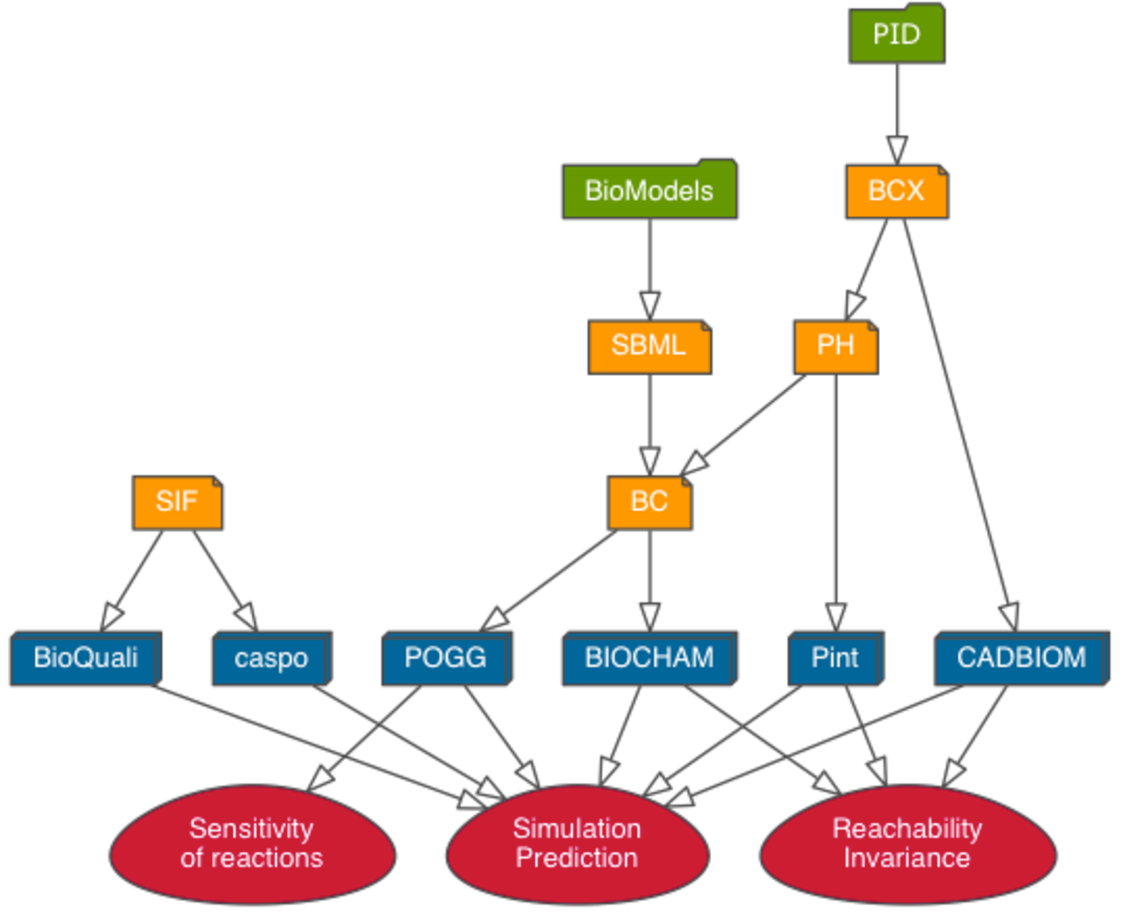
\includegraphics[width=\textwidth]{figures/biotempo-schema_global.pdf}
  }
    \caption{\label{fig:mobile} General architecture of the BIOtempo Mobyle server}
  \end{center}
\end{figure}
}

\only<2>{
\begin{figure}
  \begin{center}
  \scalebox{0.4}{
    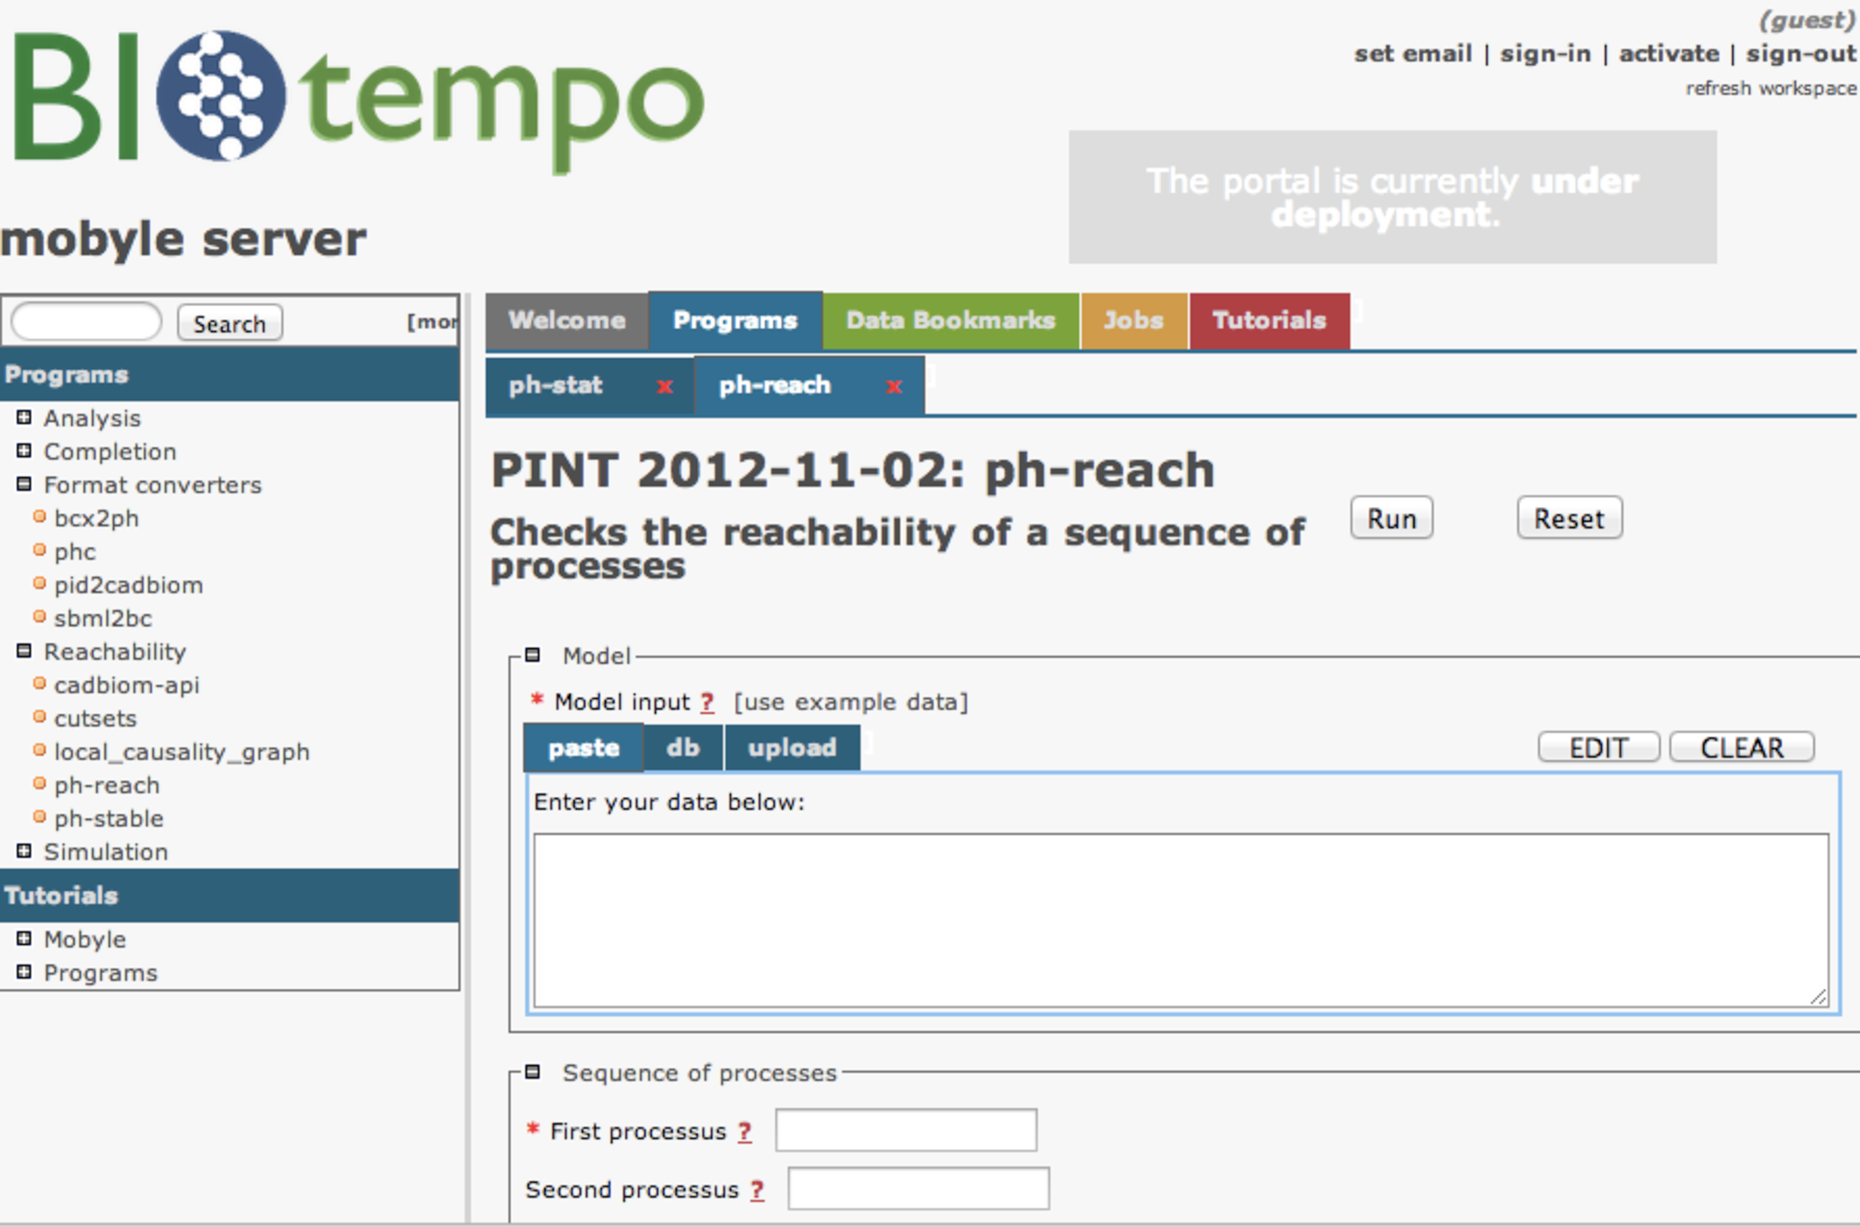
\includegraphics[width=\textwidth]{figures/biotempo-screenshot.pdf}
  }
    \caption{\label{fig:mobile} Screenshot from the BIOtempo Mobyle server: \url{http://mobyle.biotempo.univ-nantes.fr/cgi-bin/portal.py}}
  \end{center}
\end{figure}
}

\end{frame}

\section[Information inference]{Inferring information on the biological model thanks to the Process Hitting}
% Introduction à la traduction

\begin{frame}[c]
  \frametitle{Inferring a BRN with Thomas' parameters}

\begin{center}
\scalebox{\scaleinf}{
\begin{tikzpicture}
\path[use as bounding box] (-0.5,-0.8) rectangle (6.5,4);
\exphinfblack
\end{tikzpicture}
}
\end{center}

\begin{center}
\begin{tikzpicture}
\path[use as bounding box] (1,1) rectangle (4,1.5);
\only<2->{
  \path[draw] (1, 1.8) edge[->,draw,very thick] node[left=3pt,circle,draw=black,outer sep=2pt,minimum size=15pt,text=black] {1} (0, 0);}

\only<3->{
\node[circle,draw=black,inner sep=0,minimum size=5pt,fill=black] (s2) at (2,0.7) {};
\node[left=4pt of s2,circle,draw=black,outer sep=2pt,minimum size=15pt,text=black,very thick] (e2) at (2,0.8) {2};
\path[draw] (2.25, 1.8) edge[draw,very thick] (s2);
\path[draw] (1, -0.25) edge[draw,very thick] (s2);
\path[draw] (s2) edge[->,draw,very thick] (3.75, 0);}
\end{tikzpicture}
\end{center}

\begin{columns}
\begin{column}{0.6\textwidth}

\begin{center}
\begin{tikzpicture}[grn]
\path[use as bounding box] (0.5,-0.5) rectangle (2,1.5);
% Gènes noirs
\only<2->{
  \node[inner sep=0] (a) at (0,1.5) {a};
  \node[inner sep=0] (b) at (0,0) {b};
  \node[inner sep=0] (z) at (2,0.75) {z};}
% Gènes gris
\only<1>{
  \node[inner sep=0,colorgray] (a) at (0,1.5) {a};
  \node[inner sep=0,colorgray] (b) at (0,0) {b};
  \node[inner sep=0,colorgray] (z) at (2,0.75) {z};}

% Arcs colorés
\only<2->{
  \path (a) edge[act] node[elabel,above=-2pt] {$1+$} (z);
  \path (b) edge[inh] node[elabel,below=-2pt] {$1-$} (z);}
% Arcs grisés
\only<1>{
  \path (a) edge[actgray] node[elabel,above=-2pt,colorgray] {$1+$} (z);
  \path (b) edge[inhgray] node[elabel,below=-2pt,colorgray] {$1-$} (z);}
\end{tikzpicture}
\end{center}

\end{column}
\begin{column}{0.4\textwidth}

\only<1-2>{\color{colorgray}}
\begin{tabular}{c|c}
  $\omega$ & $k_{z, \omega}$ \\
\hline
  $\emptyset$ & $1$ \\
  $\{b\}$ & $0$ \\
  $\{a\}$ & $2$ \\
  $\{a;b\}$ & $1$
\end{tabular}
\vspace*{1em}

\end{column}
\end{columns}


\end{frame}

\subsection{Interaction Graph Inference}
% Inférence du Graphe des Interactions



\begin{frame}
  \frametitle{Inferring the Interaction Graph}
  \framesubtitle{\cite{Folschette2012}}

\begin{columns}
\begin{column}{0.65\textwidth}

\begin{center}\scalebox{\scaleinf}{
\only<3->{\vspace{-5em}}
\begin{tikzpicture}
  \scalebox{0.8}{
\path[use as bounding box] (-0.5,-0.8) rectangle (6.5,2.8);
\exphinf

% Processus marqués
\only<4-9>{\node[current process,fill=colorb] (hb_0) at (b_0.center) {};}
\only<5-9>{
  \node[current process,fill=colora1] (ha_1) at (a_1.center) {};
  \node[current process,fill=colora1] (hab_2) at (ab_2.center) {};}
\only<6-9>{
  \node[current process,fill=colora1] (hz_2) at (z_2.center) {};}
\only<7-9>{
  \node[current process,fill=colora0] (ha_0) at (a_0.center) {};
  \node[current process,fill=colora0] (hab_0) at (ab_0.center) {};}
\only<8-9>{
  \node[current process,fill=colora0] (hz_0) at (z_0.center) {};}

\only<10->{\node[current process,fill=colorb] (hb_1) at (b_1.center) {};}
\only<10->{
  \node[current process,fill=colora1] (ha_1) at (a_1.center) {};
  \node[current process,fill=colora1] (hab_3) at (ab_3.center) {};
  \node[current process,fill=colora0] (ha_0) at (a_0.center) {};
  \node[current process,fill=colora0] (hab_1) at (ab_1.center) {};}
\only<11->{
  \node[current process,fill=colora1] (hz_1) at (z_1.center) {};
  \node[current process,fill=colora0,inner sep=0,minimum size=7pt,draw=none] (hz_1bis) at (z_1.center) {};}

% Actions mises en valeur
\only<5-6>{
  \THit{ab_2}{}{z_1}{.north west}{z_2}
  \THit{ab_2}{}{z_0}{.west}{z_1}
  \path[bounce,bend left] \TBounce{z_1}{}{z_2}{.south} \TBounce{z_0}{}{z_1}{.south} ;}
\only<7-8>{
  \THit{ab_0}{}{z_2}{.west}{z_1}
  \THit{ab_0}{}{z_1}{.south west}{z_0}
  \path[bounce,bend right] \TBounce{z_2}{}{z_1}{.north} \TBounce{z_1}{}{z_0}{.north} ;}
\only<10->{
  \THit{ab_3}{}{z_2}{.west}{z_1}
  \THit{ab_3}{}{z_0}{.west}{z_1}
  \THit{ab_1}{}{z_2}{.west}{z_1}
  \THit{ab_1}{}{z_0}{.west}{z_1}
  \path[bounce,bend left] \TBounce{z_2}{bend right}{z_1}{.north} \TBounce{z_0}{}{z_1}{.south} ;}
}
\end{tikzpicture}
}\end{center}

\end{column}
\begin{column}{0.45\textwidth}

\begin{center}
\begin{tikzpicture}[grn]
\path[use as bounding box] (1,-0.5) rectangle (2.5,1.5);
% Gènes noirs
\only<1->{\node[inner sep=0] (a) at (0,1.5) {a};}
\only<1-3>{\node[inner sep=0] (b) at (0,0) {b};}
\only<1->{\node[inner sep=0] (z) at (2,0.75) {z};}
%\only<1-2>{\path node[elabel, below=-1em of a] {$0..1$}; \path node[elabel, below=-1em of b] {$0..1$}; \path node[elabel, below=-1em of z] {$0..2$};}
% Gènes gris
%\only<3>{\node[colorgray,inner sep=0] (a) at (0,1.5) {a};}
\only<4->{\node[colorgray,inner sep=0] (b) at (0,0) {b};}

%\newcolumntype{M}[1]{>{\raggedright}m{#1}}

% Arc noir
\only<2-12>{\path (a) edge[inf] node[elabel,above right=-2.4em,font=\scriptsize] {\begin{tabular*}{3cm}{c}%
$\color{white}\left.\color{black}\text{\begin{tabular*}{2.1cm}{l}%
  $\only<10->{\{b = 1\} \only<15>{\phantom{\Rightarrow \sim}}\only<12->{\Rightarrow {\color{exanswer}\sim}}}$\tabularnewline%
  $\only<4->{\{b = 0\} \only<9->{\Rightarrow {\color{exanswer}1+}}}$%
\end{tabular*}}\only<-16>{\right.}\only<17->{\right\}\textcolor{exanswer}{1+}}$%
\end{tabular*}} (z) ;}
\only<2-3>{\path (b) edge[inf] node[elabel, below=-2pt] {$\only<99->{-\!\only<1->{1}}$} (z) ;}
% Arc coloré
\only<13->{\path (a) edge[act,very thick,notsodarkgreen] node[elabel,above right=-2.4em,font=\scriptsize] {\begin{tabular*}{3cm}{c}%
$\color{white}\left.\color{black}\text{\begin{tabular*}{2.1cm}{l}%
  $\only<10->{\{b = 1\} \only<11>{\phantom{\Rightarrow \sim}}\only<12->{\Rightarrow {\color{exanswer}\sim}}}$\tabularnewline%
  $\only<4->{\{b = 0\} \only<9->{\Rightarrow {\color{exanswer}1+}}}$%
\end{tabular*}}\only<13->{\right\}\textcolor{exanswer}{1+}}$%
\end{tabular*}} (z) ;}
% Arcs gris
%\only<3>{\path (a) edge[inf,draw=colorgray,fill=colorgray] node[colorgray,elabel, above=-2pt] {$\only<1>{+\!\only<2->{1}}$} (z) ;}
\only<4->{\path (b) edge[inf,draw=colorgray,fill=colorgray] node[colorgray,elabel, below=-2pt] {$\only<1>{-\!\only<1->{1}}$} (z) ;}
\end{tikzpicture}
\end{center}

\end{column}
\end{columns}

\bigskip

% Méthode
\only<3-13>{
\f \tval{Exhaustive search in all possible configurations}

\pause
\begin{enumerate}[1.]
  \item Pick one regulator [\ex{$a$}], and choose an active process for all the others [\ex{$b_0$}].
\pause
  \item Change the active process of this regulator [\ex{$a_0$}, \ex{$a_1$}] and watch the \tval{focal processes}.
\pause[9]
  \item Conclude locally: ($\textcolor{colora0font}{a_0} \Rsh \textcolor{colora1font}{a_1} \Rightarrow \textcolor{colora0font}{z_0} \Rsh \textcolor{colora1font}{z_2}$)\\
      \quad $\Rightarrow \text{activation (}\textcolor{exanswer}{+}\text{) \& threshold = \ex{$1$}}$.
\pause
  \item Iterate \pause[13]and conclude globally.
\end{enumerate}
}

\only<14->{
\smallskip
\textbf{Problematic cases}:\\
\smallskip
$\left.\text{\begin{tabular}{l}
  \f No focal processes (\textbf{cycle})\\
  \f Opposite influences (\ex{$+$} \& \ex{$-$})
 \end{tabular}}\right\} \Rightarrow \text{\textbf{Unsigned edge}}$
 }
\end{frame}

\subsection{Parametrization Inference}
% Inférence de la Paramétrisation

\begin{frame}
  \frametitle{Inferring Parameters}
  \framesubtitle{\cite{Folschette2012}}

\begin{columns}
\begin{column}{0.5\textwidth}

\only<1-5>{
\begin{center}
\scalebox{0.5}{
\begin{tikzpicture}
\path[use as bounding box] (-0.5,-0.8) rectangle (6.5,2.8);
\exphinf

% Processus mis en valeur
\only<2->{
  \node[current process,fill=colorb] (hb_1) at (b_1.center) {};
  \node[current process,fill=colorb] (ha_1) at (a_1.center) {};}
\only<2->{
  \node[current process,fill=colorb] (hab_3) at (ab_3.center) {};}
\only<3->{
  \node[current process,fill=colorb] (hz_1) at (z_1.center) {};}

% Actions mises en valeur
\only<3->{
  \THit{ab_3}{}{z_2}{.west}{z_1}
  \THit{ab_3}{}{z_0}{.west}{z_1}
  \path[bounce,bend left] \TBounce{z_2}{bend right}{z_1}{.north} \TBounce{z_0}{}{z_1}{.south};}
\end{tikzpicture}
}
\end{center}
}

%\only<4->{
%\begin{center}
%\scalebox{0.5}{
%\begin{tikzpicture}
%\path[use as bounding box] (-0.5,-0.8) rectangle (6.5,2.8);
%\exphinfprojssc
%
%% Processus mis en valeur
%\only<2->{
%  \node[current process,fill=colorb] (hb_1) at (b_1.center) {};
%  \node[current process,fill=colorb] (ha_1) at (a_1.center) {};}
%
%% Actions mises en valeur
%\only<2->{
%  \THit{a_1}{}{z_0}{.west}{z_1}
%  \THit{a_1}{}{z_1}{.north west}{z_2}
%  \THit{b_1}{}{z_1}{.south west}{z_0}
%  \THit{b_1}{}{z_2}{.west}{z_1}
%  \path[bounce,bend left] \TBounce{z_0}{}{z_1}{.south} \TBounce{z_1}{}{z_2}{.south}
%    \TBounce{z_1}{bend right}{z_0}{.north} \TBounce{z_2}{bend right}{z_1}{.north} ;}
%}
%\end{tikzpicture}
%\end{center}
%}

\end{column}
\begin{column}{0.2\textwidth}

\begin{center}
\begin{tikzpicture}[grn]
\path[use as bounding box] (0.5,-0.5) rectangle (2,1.5);
% Gènes noirs
  \node[inner sep=0] (a) at (0,1.5) {a};
  \node[inner sep=0] (b) at (0,0) {b};
  \node[inner sep=0] (z) at (2,0.75) {z};
% Arcs colorés
  \path (a) edge[act] node[elabel,above=-2pt] {$1+$} (z) ;
  \path (b) edge[inh] node[elabel,below=-2pt] {$1-$} (z) ;
\end{tikzpicture}
\end{center}

\end{column}
\begin{column}{0.25\textwidth}

\only<1-5>{
\begin{tabular}{c|c|c}
%  $\omega$ & $k_{z, \omega}$ \\
%\hline
  \multicolumn{2}{c|}{$\omega$} & \multirow{2}{*}{$k_{z, \omega}$} \\
\cline{1-2}
  $a$ & $b$ & \\
\hline
  \only<2->{\color{colorgray}}$-$ & \only<2->{\color{colorgray}}$+$ & \\
  \only<2->{\color{colorgray}}$-$ & \only<2->{\color{colorgray}}$-$ & \\
  \only<2->{\color{colorgray}}$+$ & \only<2->{\color{colorgray}}$+$ & \\
  \only<1>{$+$}\only<2->{\redex{$+$}} & \only<1>{$-$}\only<2->{\redex{$-$}} & \uncover<4->{\redex{$1$}}
\end{tabular}
}

\end{column}
\end{columns}

\smallskip
\pause[2]
\begin{enumerate}[1.]
  \item For each configuration of resources \quad [\ex{$\omega = \{a^+, b^-\}$}]\\
\pause
        find the \tval{focal processes}.\pause[4] If possible, conclude. \quad [$\ex{k_{z,\{a^+, b^-\}} = 1}$]
\pause[5]
 \item[] Inconclusive cases:
  \begin{itemize}
    \item[--] Behavior cannot be represented as a BRN
    \item[--] Lack of cooperation (no focal processes)
  \end{itemize}
\end{enumerate}
\end{frame}

\begin{frame}
  \frametitle{Inferring Parameters}
%  \framesubtitle{\tcite{PMR10-TCSB}}

\begin{columns}
\begin{column}{0.5\textwidth}

\begin{center}
\scalebox{0.5}{
\begin{tikzpicture}
\path[use as bounding box] (-0.5,-0.8) rectangle (6.5,2.8);
\exphinfprojssc

% Processus mis en valeur
  \node[current process,fill=colorb] (hb_1) at (b_1.center) {};
  \node[current process,fill=colorb] (ha_1) at (a_1.center) {};
%
%% Actions mises en valeur
  \THit{a_1}{}{z_0}{.west}{z_1}
  \THit{a_1}{}{z_1}{.north west}{z_2}
  \THit{b_1}{}{z_1}{.south west}{z_0}
  \THit{b_1}{}{z_2}{.west}{z_1}
  \path[bounce,bend left] \TBounce{z_0}{}{z_1}{.south} \TBounce{z_1}{}{z_2}{.south}
    \TBounce{z_1}{bend right}{z_0}{.north} \TBounce{z_2}{bend right}{z_1}{.north} ;
\end{tikzpicture}
}
\end{center}
%
\end{column}
\begin{column}{0.2\textwidth}
%
\begin{center}
\begin{tikzpicture}[grn]
\path[use as bounding box] (0.5,-0.5) rectangle (2,1.5);
% Gènes noirs
  \node[inner sep=0] (a) at (0,1.5) {a};
  \node[inner sep=0] (b) at (0,0) {b};
  \node[inner sep=0] (z) at (2,0.75) {z};
% Arcs colorés
  \path (a) edge[act] node[elabel,above=-2pt] {$1+$} (z) ;
  \path (b) edge[inh] node[elabel,below=-2pt] {$1-$} (z) ;
\end{tikzpicture}
\end{center}

\end{column}
\begin{column}{0.25\textwidth}

\begin{tabular}{c|c|c}
%  $\omega$ & $k_{z, \omega}$ \\
%\hline
  \multicolumn{2}{c|}{$\omega$} & \multirow{2}{*}{$k_{z, \omega}$} \\
\cline{1-2}
  $a$ & $b$ & \\
\hline
  $-$ & $+$ & \redex{\textit{?}} \\ %\textcolor{lightgray}{\textit{?}} \\
  $-$ & $-$ & $0$ \\
  $+$ & $+$ & $2$ \\
  $+$ & $-$ & \redex{\textit{?}} %\textcolor{lightgray}{\textit{?}}
\end{tabular}
%
\end{column}
\end{columns}

\smallskip
\begin{enumerate}[1.]
  \item For each configuration of resources \quad [\ex{$\omega = \{a^+, b^-\}$}]\\
        find the \tval{focal processes}. If possible, conclude. \quad [$\ex{k_{z,\{a^+, b^-\}} = 1}$]
 \item[] Inconclusive cases:
  \begin{itemize}
    \item[--] Behavior cannot be represented as a BRN
    \item[--] Lack of cooperation (no focal processes)
  \end{itemize}
\medskip
  \item If some parameters could not be inferred, enumerate all admissible parametrizations, regarding \textbf{biological constraints} and \textbf{the dynamics of the Process Hitting} $\Rightarrow$ $k_{z, \{a^+, b^-\}} \in \{0 ; 1 ; 2\}$; $k_{z, \{a^-, b^+\}} \in \{0 ; 1 ; 2\}$
\end{enumerate}
\end{frame}

\section{Summary \& Conclusion}
% Performances et conclusion


\begin{frame}[c]
  \frametitle{Implementation}

\small
\tval{Workflow}:
\begin{itemize}
  \item Read and translate the models with \tval{OCaml}\\
        \quad\f Uses the existing free library \tval{Pint}\\
        \quad\f Documentation + examples: \footnotesize\url{http://loicpauleve.name/pint}
  \item Express the problem in \tval{ASP} (logic programming)\\
        \quad\f Solve with \tval{Clingo} (\tval{Gringo} + \tval{Clasp})
\end{itemize}

\pause
\bigskip
\footnotesize
\begin{tabular}{c||r@{+}l|c|c||c|c||c|c|}
\multicolumn{5}{c||}{Model specifications} & \multicolumn{2}{c||}{IG inference} & \multicolumn{2}{c|}{Parameters inference}\\
\hline
\tval{Name} & S & CS & P & A & $\Delta t$ & Edges & $\Delta t$ & Parameters\\
\hline
  \tval{\ex{[EGFR20]}} & \tval{20} & 22 & 152 & 399 & \tval{1s} & 50 & \tval{1s} & 191\\
\hline
  \tval{\ex{[TCRSIG40]}} & \tval{40} & 14 & 156 & 301 & \tval{1s} & 54 & \tval{1s} & 143\\
\hline
  \tval{\ex{[TCRSIG94]}} & \tval{94} & 39 & 448 & 1124 & \tval{13s} & 169 & $\infty$ & $2.10^9$\\
\hline
  \tval{\ex{[EGFR104]}} & \tval{104} & 89~ & 748 & 2356 & \tval{4min} & 241 & \tval{1min 30s} & $1.10^6 / 2.10^6$\\
\hline
\end{tabular}

S = Sorts \quad CS = Cooperative sorts \quad P = Processes \quad A = Actions

\bigskip
\quad\tval{\ex{[EGFR20]}}: Epidermal Growth Factor Receptor, by \"Ozg\"ur Sahin et al.\\
\quad\tval{\ex{[EGFR104]}}: Epidermal Growth Factor Receptor, by Regina Samaga et al.\\
\quad\tval{\ex{[TCRSIG40]}}: T-Cell Receptor Signaling, by Steffen Klamt et al.\\
\quad\tval{\ex{[TCRSIG94]}}: T-Cell Receptor Signaling, by Julio Saez-Rodriguez et al.

\end{frame}



\begin{frame}[c]
  \frametitle{Summary}

\only<1>{
\begin{block}{Process Hitting and ASP}
\begin{itemize}
  \item Inference of the \tval{complete Interaction Graph}
  \item Inference of the \tval{possibly partial Parametrization}
  \item Enumerate all full \& \tval{admissible Parametrizations}
\end{itemize}
\quad\quad\f Exhaustive approaches
\end{block}

\bigskip
\tval{Complexity}: linear in the number of genes, exponential in the number of regulators of one gene

}

\only<2>{
\begin{block}{Contribution: new translation Process Hitting $\rightsquigarrow$ Ren\'e Thomas}
\begin{fleches}
  \item New \tval{formal link} between the two models
  \item More \tval{visibility} to the Process Hitting
  \item Inference approach that takes benefit from both the Process Hitting compact structure and the power of ASP 
\end{fleches}
\end{block}
}

\end{frame}

\frame{\frametitle{Further work}

\begin{alertblock}{Models and algorithms}
\begin{itemize}
\item Add \textbf{priorities} in the Process Hitting framework and adapt the static analyses approaches for this enriched model \cite{FolschetteCS2Bio13} 
\item From priorities to \textbf{quantitative timing information}
\item Connect Process Hitting compact structure with \textbf{decomposition techniques} in continuous approaches \cite{ammarreduction2012, ChancellorACMR13}
\end{itemize}
\end{alertblock}

\begin{block}{Application}
\begin{itemize}
\item Use the approach for the analysis of \textbf{larger} biological networks 
\item Contribute to the \textbf{discovery} of biological regulatory networks based on biological data 
\item Study key properties (e.g. concept of \textbf{resilience})
\end{itemize}
\end{block}

}

\appendix

% On veut un style <<alpha>>
\bibliography{biblio}
\bibliographystyle{alpha}

\end{document}